%\documentclass[12pt]{article}

\questionheader{ex:s2.4}


%%%%%%%%%%%%%%%%%%
\subsection*{\Conceptual}
%%%%%%%%%%%%%%%%%%

%%%%%%%%%%%%%%%%%%%%%%%%%%%%%%%%
\begin{question}
Write out the chain rule
for each of the following functions.
\begin{enumerate}[(a)]
\item
   $\pdiff{h}{x}$ for $h(x,y)=f\big(x,u(x,y)\big)$
\item
   $\diff{h}{x}$ for $h(x)=f\big(x,u(x),v(x)\big)$
\item
   $\pdiff{h}{x}$ for $h(x,y,z)=f\big(u(x,y,z),v(x,y),w(x)\big)$
\end{enumerate}
\end{question}

\begin{hint}
 Review   \S\eref{CLP200}{subsec memory aid} in the CLP-3 text.
\end{hint}

\begin{answer}
(a) $\pdiff{h}{x}(x,y)
=\pdiff{f}{x}\big(x,u(x,y)\big)
+\pdiff{f}{u}\big(x,u(x,y)\big)
\pdiff{u}{x}(x,y)$

(b) $\diff{h}{x}(x)
=\pdiff{f}{x}\big(x,u(x),v(x)\big)
+\pdiff{f}{u}\big(x,u(x),v(x)\big)
\diff{u}{x}(x)
+\pdiff{f}{v}\big(x,u(x),v(x)\big)
\diff{v}{x}(x)$

(c) $\pdiff{h}{x}(x,y,z)
=\pdiff{f}{u}\big(u(x,y,z),v(x,y),w(x)\big)
\pdiff{u}{x}(x,y,z)
+\pdiff{f}{v}\big(u(x,y,z),v(x,y),w(x)\big)
\pdiff{v}{x}(x,y)$ 
\null$\ \ \ \ \ \ \ \ +\pdiff{f}{w}\big(u(x,y,z),v(x,y),w(x)\big)
\diff{w}{x}(x)$


\end{answer}

\begin{solution}

(c) We'll start with part (c) and follow the procedure given in 
\S\eref{CLP200}{subsec memory aid} in the CLP-3 text. We are to compute the
derivative of $h(x,y,z)=f\big(u(x,y,z),v(x,y),w(x)\big)$ with respect to 
$x$. For this function, the template of Step 2 in 
\S\eref{CLP200}{subsec memory aid} is
\begin{equation*}
\pdiff{h}{x}=\frac{\partial f}{ }\frac{ }{\partial x}
\end{equation*}
Note that 
\begin{itemize}
\item
The function $h$ appears once in the numerator on the left.
The function $f$, from which $h$ is constructed by a change of variables,
appears once in the numerator on the right.

\item
The variable, $x$, in the denominator on the left appears once in the
denominator on the right. 
\end{itemize}
Now we fill in the blanks with every variable that makes sense. In 
particular, since $f$ is a function of $u$, $v$ and $w$, it may only be 
differentiated with respect to $u$, $v$ and $w$. So we add together
three copies of our template --- one for each of $u$, $v$ and $w$:
\begin{align*}
\pdiff{h}{x}=\pdiff{f}{u}\pdiff{u}{x}
             +\pdiff{f}{v}\pdiff{v}{x}
             +\pdiff{f}{w}\diff{w}{x}
\end{align*}
Since $w$ is a function of only one variable, we use the ordinary 
derivative symbol $\diff{w}{x}$, rather than the partial
derivative symbol $\pdiff{w}{x}$ in the third copy.
Finally we put in the only functional dependence that makes sense. 
The left hand side is a function of $x$, $y$ and $z$, because $h$
is a function of $x$, $y$ and $z$. Hence the right hand side must 
also be a function of $x$, $y$ and $z$. As $f$ is a
function of $u$, $v$ and $w$, this is achieved by evaluating $f$ at 
$u=u(x,y,z)$, $v=v(x,y)$ and $w=w(x)$.
\begin{align*}
\pdiff{h}{x}(x,y,z)
&=\pdiff{f}{u}\big(u(x,y,z),v(x,y),w(x)\big)
\pdiff{u}{x}(x,y,z)
+\pdiff{f}{v}\big(u(x,y,z),v(x,y),w(x)\big)
\pdiff{v}{x}(x,y) \\&\hskip2in
+\pdiff{f}{w}\big(u(x,y,z),v(x,y),w(x)\big)
\diff{w}{x}(x)
\end{align*}

(a)
We again follow the procedure given in 
\S\eref{CLP200}{subsec memory aid} in the CLP-3 text. We are to compute the
derivative of $h(x,y)=f\big(x,u(x,y)\big)$ with respect to 
$x$. For this function, the template of Step 2 in 
\S\eref{CLP200}{subsec memory aid} is
\begin{equation*}
\pdiff{h}{x}=\frac{\partial f}{ }\frac{ }{\partial x}
\end{equation*}
Now we fill in the blanks with every variable that makes sense. In 
particular, since $f$ is a function of $x$ and $u$, it may only be 
differentiated with respect to $x$, and $u$. So we add together
two copies of our template --- one for $x$ and one for $u$:
\begin{align*}
\pdiff{h}{x}=\pdiff{f}{x}\diff{x}{x}
             +\pdiff{f}{u}\pdiff{u}{x}
\end{align*}
In $\diff{x}{x}$ we are to differentiate the (explicit) function $x$
(i.e. the function $F(x)=x$) with respect to $x$. The answer is of 
course $1$. So 
\begin{align*}
\pdiff{h}{x}=\pdiff{f}{x}
             +\pdiff{f}{u}\diff{u}{x}
\end{align*} 
Finally we put in the only functional depedence that makes sense. 
The left hand side is a function of $x$, and $y$, because $h$
is a function of $x$ and $y$. Hence the right hand side must 
also be a function of $x$ and $y$. As $f$ is a
function of $x$, $u$, this is achieved by evaluating $f$ at 
$u=u(x,y)$.
\begin{align*}
\pdiff{h}{x}(x,y)
=\pdiff{f}{x}\big(x,u(x,y)\big)
+\pdiff{f}{u}\big(x,u(x,y)\big)
\pdiff{u}{x}(x,y)
\end{align*}


(b) Yet again we follow the procedure given in 
\S\eref{CLP200}{subsec memory aid} in the CLP-3 text. We are to compute the
derivative of $h(x)=f\big(x,u(x),v(x)\big)$ with respect to 
$x$. For this function, the template of Step 2 in 
\S\eref{CLP200}{subsec memory aid} is
\begin{equation*}
\diff{h}{x}=\frac{\partial f}{ }\frac{ }{\partial x}
\end{equation*}
(As $h$ is function of only one variable, we use the ordinary derivative
symbol $\diff{h}{x}$ on the left hand side.)
Now we fill in the blanks with every variable that makes sense. In 
particular, since $f$ is a function of $x$, $u$ and $v$, it may only be 
differentiated with respect to $x$, $u$ and $v$. So we add together
three copies of our template --- one for each of $x$, $u$ and $v$:
\begin{align*}
\diff{h}{x}&=\pdiff{f}{x}\diff{x}{x}
             +\pdiff{f}{u}\diff{u}{x}
             +\pdiff{f}{v}\diff{v}{x} \\
            &=\pdiff{f}{x}
             +\pdiff{f}{u}\diff{u}{x}
             +\pdiff{f}{v}\diff{v}{x}
\end{align*}
Finally we put in the only functional depedence that makes sense. 
\begin{align*}
\diff{h}{x}(x)
=\pdiff{f}{x}\big(x,u(x),v(x)\big)
+\pdiff{f}{u}\big(x,u(x),v(x)\big)
\diff{u}{x}(x)
+\pdiff{f}{v}\big(x,u(x),v(x)\big)
\diff{v}{x}(x)
\end{align*}

\end{solution}
%%%%%%%%%%%%%%%%%%%%%%%%%%%%%%%%
\begin{question}A piece of the surface $z=f(x,y)$ is shown below for some continuously differentiable function $f(x,y)$. The level curve $f(x,y)=z_1$ is marked with a blue line. The three points $P_0$, $P_1$, and $P_2$ lie on the surface.
	
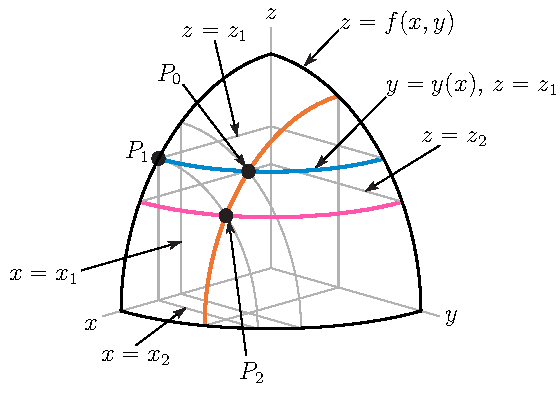
\includegraphics{fig/partialTotalX.pdf}
	
	On the level curve $z=z_1$, we can think of $y$ as a function of $x$. Let $w(x)=f(x,y(x))=z_1$. We approximate, at $P_0$, $f_x(x,y) \approx \frac{\Delta f}{\Delta x}$ and $\frac{dw}{dx}(x)\approx\frac{\Delta w}{\Delta x}$. Identify the quantities $\Delta f$, $\Delta w$, and $\Delta x$ from the diagram.% Describe also when $\Delta y=0$ or $\Delta z =0$.
	
\end{question}
\begin{hint}
%text ex 2.4.10
This is a visualization, in a simplified setting, of Example~\eref{CLP3}{eg:chainRuleE} in CLP3.
\end{hint}
\begin{answer}
	
\textit{To visualize, in a simplified setting, the situation from Example~\eref{CLP3}{eg:chainRuleE} in CLP3, note that $w'(x)$ is the rate of change of $z$ as we slide along the blue line, while $f_x(x,y)$ is the change of $z$ as we slide along the orange line.}
	
In the approximation $f_x(x,y)\approx \frac{\Delta f}{\Delta x}$, starting at the point $P_0$, $\Delta x=x_2-x_1$ and $\Delta f=z_2-z_1$.

In the approximation $\diff{w}{x}\approx \frac{\Delta w}{\Delta x}$, starting at the point $P_0$,  $\Delta x=x_2-x_1$ again, and $\Delta w=z_1-z_1=0$.

\end{answer}
\begin{solution}
	
\textit{To visualize, in a simplified setting, the situation from Example~\eref{CLP3}{eg:chainRuleE} in CLP3, note that $w'(x)$ is the rate of change of $z$ as we slide along the blue line, while $f_x(x,y)$ is the change of $z$ as we slide along the orange line.}

In the partial derivative $f_x(x,y)\approx \frac{\Delta f}{\Delta x}$, we let $x$ change, while $y$ stays the same. Necessarily, that forces $f$ to change as well. Starting at point $P_0$, if we move $x$ but keep $y$ fixed, we end up at $P_2$. According to the labels on the diagram, $\Delta x$ is $x_2-x_1$, and $\Delta f$ is $z_2-z_1$.


The function $w(x)$ is a constant function, so we expect $w'(x)=0$.
In the approximation $\diff{w}{x}\approx \frac{\Delta w}{\Delta x}$, we let $x$ change, but $w$ stays the same. Necessarily, to stay on the surface, this
forces $y$ to change. Starting at point $P_0$, if we move $x$ but keep 
$z=f(x,y)$ fixed, we end up at $P_1$. According to the labels on the diagram, $\Delta x$ is $x_2-x_1$ again, and $\Delta w=z_1-z_1=0$.

To compare the two situations, note the first case has $\Delta y =0$ while 
the second case has $\Delta f =0$.
\end{solution}
%%%%%%%%%%%%%%%%%%%%%%%%%%%%%%%%
\begin{question}[M200 2000D] %8
Let $w=f(x,y,t)$ with $x$ and $y$ depending on $t$. Suppose
that at some point $(x,y)$ and at some time $t$, the partial derivatives
$f_x$, $f_y$ and $f_t$ are equal to $2$, $-3$ and $5$ respectively, while
$\diff{x}{t}=1$ and $\diff{y}{t}=2$. Find and explain the difference
between $\diff{w}{t}$ and $f_t$.
\end{question}

\begin{hint}
Pay attention to which variables change, and which are held fixed, in each context.
\end{hint}

\begin{answer}
$\diff{w}{t}=1$ and $f_t=5$. 
$f_t$ gives the rate of change of $f(x,y,t)$ as $t$ varies 
while $x$ and $y$ are held fixed. 
$\diff{w}{t}$ gives the rate of change of $f\big(x(t),y(t),t\big)$.
For the latter all of $x=x(t)$, $y=y(t)$ and $t$ are 
changing at once.
\end{answer}

\begin{solution}
We are told in the statement of the question that 
$w(t)= f\big(x(t),y(t),t\big)$.
Applying the chain rule to
$
w(t)= f\big(x(t),y(t),t\big),
$
by following the procedure given in 
\S\eref{CLP200}{subsec memory aid} in the CLP-3 tex, gives
\begin{align*}
\diff{w}{t}(t)
    &=\pdiff{f}{x}\big(x(t),y(t),t\big)\diff{x}{t}(t)
    +\pdiff{f}{y}\big(x(t),y(t),t\big)\diff{y}{t}(t)
    +\pdiff{f}{t}\big(x(t),y(t),t\big)\diff{t}{t} \\
   &=\pdiff{f}{x}\big(x(t),y(t),t\big)\diff{x}{t}(t)
    +\pdiff{f}{y}\big(x(t),y(t),t\big)\diff{y}{t}(t)
    +\pdiff{f}{t}\big(x(t),y(t),t\big)
\end{align*}
Substituting in the values given in the question
\begin{equation*}
\diff{w}{t}
    =2\times 1
    -3\times 2
    +5
    =1
\end{equation*}
On the other hand, we are told explicitly in the question that $f_t$ is $5$.
The reason that $f_t$ and $\diff{w}{t}$ are different is that
\begin{itemize}\itemsep1pt \parskip0pt \parsep0pt %\itemindent-15p
\item
$f_t$ gives the rate of change of $f(x,y,t)$ as $t$ varies 
while $x$ and $y$ are held fixed, but
\item
$\diff{w}{t}$ gives the rate of change of $f\big(x(t),y(t),t\big)$.
For the latter all of $x=x(t)$, $y=y(t)$ and $t$ are 
changing at once.
\end{itemize}
\end{solution}

%%%%%%%%%%%%%%%%%%%%%%%%%%%%%%%%
\begin{question}
Thermodynamics texts
use the relationship 
\begin{equation*}
\left(\pdiff{y}{x}\right)
\left(\pdiff{z}{y}\right)
\left(\pdiff{x}{z}\right)=-1
\end{equation*}
Explain the meaning of this equation and prove that it is true.
\end{question}

\begin{hint}
The basic assumption is that the three quantites $x$, $y$
and $z$ are not independent. Given any two of them, the third is uniquely
determined. They are assumed to satisfy a relationship
$F(x,y,z)=0$, which can be solved to
\begin{itemize}\itemsep1pt \parskip0pt \parsep0pt %\itemindent-15p
\item
determine $x$ as a function of $y$ and $z$ (say $x=f(y,z)$) and 
can alternatively be solved to
\item
determine $y$ as a function of $x$ and $z$ (say $y=g(x,z)$) and 
can alternatively be solved to
\item
determine $z$ as a function of $x$ and $y$
(say $z=h(x,y)$). 
\end{itemize}
For example, saying that  $F(x,y,z)=0$ determines $x=f(y,z)$ means that 
\begin{equation*}
F\big(f(y,z),y,z\big)=0
\tag{$*$}
\end{equation*}
for all $y$ and $z$. The equation 
\begin{equation*}
\left(\pdiff{y}{x}\right)
\left(\pdiff{z}{y}\right)
\left(\pdiff{x}{z}\right)=-1
\end{equation*}
really means
\begin{equation*}
\left(\pdiff{g}{x}\right)
\left(\pdiff{h}{y}\right)
\left(\pdiff{f}{z}\right)=-1
\end{equation*}
So use $(*)$ to compute $\pdiff{f}{z}$.  Use other equations similar to $(*)$
to compute $\pdiff{g}{x}$ and $\pdiff{h}{y}$.
\end{hint}

\begin{answer}
See the solution.
\end{answer}

\begin{solution}
 The basic assumption is that the three quantites $x$, $y$
and $z$ are not independent. Given any two of them, the third is uniquely
determined. They are assumed to satisfy a relationship
$F(x,y,z)=0$, which can be solved to
\begin{itemize}\itemsep1pt \parskip0pt \parsep0pt %\itemindent-15p
\item
determine $x$ as a function of $y$ and $z$ (say $x=f(y,z)$) and 
can alternatively be solved to
\item
determine $y$ as a function of $x$ and $z$ (say $y=g(x,z)$) and 
can alternatively be solved to
\item
determine $z$ as a function of $x$ and $y$
(say $z=h(x,y)$). 
\end{itemize}
As an example, if $F(x,y,z) = xyz-1$, then 
\begin{itemize}\itemsep1pt \parskip0pt \parsep0pt %\itemindent-15p
\item
$F(x,y,z)=xyz-1=0$ implies that $x=\frac{1}{yz}=f(y,z)$ and
\item
$F(x,y,z)=xyz-1=0$ implies that $y=\frac{1}{xz}=g(x,z)$ and
\item
$F(x,y,z)=xyz-1=0$ implies that $z=\frac{1}{xy}=h(x,y)$
\end{itemize}
In general, saying that  $F(x,y,z)=0$ determines $x=f(y,z)$ means that 
\begin{equation*}
F\big(f(y,z),y,z\big)=0
\tag{$*$}
\end{equation*}
for all $y$ and $z$. 
Set $\mathcal{F}(y,z)=F\big(f(y,z),y,z\big)$. Applying the chain rule to
$\mathcal{F}(y,z)=F\big(f(y,z),y,z\big)$ (with $y$ and $z$ independent variables) 
gives
\begin{align*}
\pdiff{\mathcal{F}}{z}(y,z) 
%&= \pdiff{F}{x}\big(f(y,z),y,z\big)\pdiff{f}{z}(y,z)
%+\pdiff{F}{z}\big(f(y,z),y,z\big)\diff{z}{z} \\
&= 
\pdiff{F}{x}\big(f(y,z),y,z\big)
\pdiff{f}{z}(y,z)
+\pdiff{F}{z}\big(f(y,z),y,z\big)
\end{align*}
The equation $(*)$ says that $\mathcal{F}(y,z)=F\big(f(y,z),y,z\big)=0$ 
for all $y$ and $z$.
So differentiating the equation $(*)$ with respect to 
$z$ gives
\begin{align*}
\pdiff{\mathcal{F}}{z}(y,z)&=\pdiff{F}{x}\big(f(y,z),y,z\big)
\pdiff{f}{z}(y,z)
+\pdiff{F}{z}\big(f(y,z),y,z\big)=0 \\
&\implies
\pdiff{f}{z}(y,z)
=-\frac{\pdiff{F}{z}\big(f(y,z),y,z\big)}
{\pdiff{F}{x}\big(f(y,z),y,z\big)}
\end{align*}
for all $y$ and $z$. Similarly, differentiating 
$F\big(x,g(x,z),z\big)=0$ with respect to $x$ and
$F\big(x,y,h(x,y)\big)=0$ with respect to $y$ gives
\begin{align*}
\pdiff{g}{x}(x,z)
=-\frac{\pdiff{F}{x}\big(x,g(x,z),z\big)}
{\pdiff{F}{y}\big(x,g(x,z),z\big)}\qquad
\pdiff{h}{y}(x,y)
=-\frac{\pdiff{F}{y}\big(x,y,h(x,y)\big)}
{\pdiff{F}{z}\big(x,y,h(x,y)\big)}
\end{align*}
If $(x,y,z)$ is any point satisfying $F(x,y,z)=0$ 
(so that $x=f(y,z)$ and $y=g(x,z)$ and  $z=h(x,y)$), then
\begin{align*}
\pdiff{f}{z}(y,z)
=-\frac{\pdiff{F}{z}\big(x,y,z\big)}
{\pdiff{F}{x}\big(x,y,z\big)}\qquad
\pdiff{g}{x}(x,z)
=-\frac{\pdiff{F}{x}\big(x,y,z\big)}
{\pdiff{F}{y}\big(x,y,z\big)}\qquad
\pdiff{h}{y}(x,y)
=-\frac{\pdiff{F}{y}\big(x,y,z\big)}
{\pdiff{F}{z}\big(x,y,z\big)}
\end{align*}
and
\begin{align*}
\pdiff{f}{z}(y,z)\ 
\pdiff{g}{x}(x,z)\ 
\pdiff{h}{y}(x,y)
&=-\frac{\pdiff{F}{z}\big(x,y,z\big)}
{\pdiff{F}{x}\big(x,y,z\big)}\ 
\frac{\pdiff{F}{x}\big(x,y,z\big)}
{\pdiff{F}{y}\big(x,y,z\big)}\ 
\frac{\pdiff{F}{y}\big(x,y,z\big)} 
{\pdiff{F}{z}\big(x,y,z\big)} \\
&=-1
\end{align*}
\end{solution}


%%%%%%%%%%%%%%%%%%%%%%%%%%%%%%%%
\begin{question}
What is wrong with the following argument? Suppose that $w=f(x,y,z)$
and $z=g(x,y)$. By the chain rule,
\begin{align*}
\pdiff{w}{x}
=\pdiff{w}{x}\pdiff{x}{x}
+\pdiff{w}{y}\pdiff{y}{x}
+\pdiff{w}{z}\pdiff{z}{x}
=\pdiff{w}{x}
+\pdiff{w}{z}\pdiff{z}{x}
\end{align*}
Hence $0=\pdiff{w}{z}\pdiff{z}{x}$
and so $\pdiff{w}{z}=0$
or $\pdiff{z}{x}=0$.
\end{question}

\begin{hint}
Is the $\pdiff{w}{x}$ on the left hand side really
the same as the $\pdiff{w}{x}$ on the right hand side?
\end{hint}

\begin{answer}
The problem is that $\pdiff{w}{x}$ is used to represent
two completely different functions in the same equation.
See the solution for more details.
\end{answer}

\begin{solution}
The problem is that $\pdiff{w}{x}$ is used
to represent
two completely different functions in the same equation. The careful way
to write the equation is the following. Let $f(x,y,z)$
and $g(x,y)$ be continuously differentiable functions and define
$w(x,y)=f\big(x,y,g(x,y)\big)$. By the chain rule,
\begin{align*}
\pdiff{w}{x}(x,y)
&=\pdiff{f}{x}\big(x,y,g(x,y)\big)
\pdiff{x}{x}
+\pdiff{f}{y}\big(x,y,g(x,y)\big)
\pdiff{y}{x}
+\pdiff{f}{z}\big(x,y,g(x,y)\big)
\pdiff{g}{x}(x,y)\cr
&=\pdiff{f}{x}\big(x,y,g(x,y)\big)
+\pdiff{f}{z}\big(x,y,g(x,y)\big)
\pdiff{g}{x}(x,y)
\end{align*}
While $w(x,y)=f\big(x,y,g(x,y)\big)$, it is not true that
$\pdiff{w}{x}(x,y)
=\pdiff{f}{x}\big(x,y,g(x,y)\big)$.
For example, take $f(x,y,z)=x-z$ and $g(x,y)=x$. Then 
$w(x,y)=f\big(x,y,g(x,y)\big)=x-g(x,y)=0$ for all $(x,y)$, so that 
$\pdiff{w}{x}(x,y)=0$
while $\pdiff{f}{x}(x,y,z)=1$ for all $(x,y,z)$.
\end{solution}


%%%%%%%%%%%%%%%%%%%%%%%%%%%%
%\Instructions{Questions~\ref{prob_s1.0first} through \ref{prob_s1.0last} provide practice with.}
%%%%%%%%%%%%%%%%%%%%

%%%%%%%%%%%%%%%%%%
\subsection*{\Procedural}
%%%%%%%%%%%%%%%%%%

%%%%%%%%%%%%%%%%%%%%%%%%%%%%%%%%
\begin{question}
Use two methods (one using the chain rule) to evaluate 
$\pdiff{w}{s}$ and $\pdiff{w}{t}$ 
given that the function $w=x^2+y^2+z^2$, with 
$x=st,\ y=s\cos t$ and $z=s\sin t$.
\end{question}

\begin{hint}
To avoid the chain rule, write $w$ explicitly as a function of $s$ and $t$.
\end{hint}

\begin{answer}
$w_s(s,t)=2s(t^2+1)$\qquad
$w_t(s,t)=s^2(2t)$
\end{answer}

\begin{solution}
\emph{Method 1:}
Since $w(s,t)=x(s,t)^2+y(s,t)^2+z(s,t)^2$ with $x(s,t)=st$, 
$y(s,t)=s\cos t$ and $z(s,t)=s\sin t$ we can write out $w(s,t)$
explicitly:
\begin{align*}
w(s,t)&=(st)^2+(s\cos t)^2+(s\sin t)^2
      =s^2(t^2+1)\\
\implies w_s(s,t)&=2s(t^2+1)\qquad\text{and}\qquad
  w_t(s,t)=s^2(2t)
\end{align*}

\emph{ Method 2:}
The question specifies that $w(s,t)=x(s,t)^2+y(s,t)^2+z(s,t)^2$ with 
$x(s,t)=st$, $y(s,t)=s\cos t$ and $z(s,t)=s\sin t$. That is, 
$w(s,t) = W\big(x(s,t), y(s,t), z(s,t)\big)$
with $W(x,y,z)= x^2+y^2+z^2$. Applying the chain rule to $w(s,t) = W\big(x(s,t), y(s,t), z(s,t)\big)$ and noting that $\pdiff{W}{x}=2x$,
$\pdiff{W}{y}=2y$, $\pdiff{W}{z}=2z$, gives
\begin{align*}
 \pdiff{w}{s}(s,t)
 &= \pdiff{W}{x}\big(x(s,t), y(s,t), z(s,t)\big)\pdiff{x}{s}(s,t)
   + \pdiff{W}{y}\big(x(s,t), y(s,t), z(s,t)\big)\pdiff{y}{s}(s,t)\\&\hskip1in
   + \pdiff{W}{z}\big(x(s,t), y(s,t), z(s,t)\big)\pdiff{z}{s}(s,t) \\
 &=2 x(s,t)\ x_s(s,t)+2 y(s,t)\ y_s(s,t)+2 z(s,t)\ z_s(s,t) \\
                  &=2 (st)\ t+2 (s\cos t)\ \cos t+2 (s\sin t)\ \sin t\\
                 &=2 st^2+2 s\\
  \pdiff{w}{t}(s,t)
 &= \pdiff{W}{x}\big(x(s,t), y(s,t), z(s,t)\big)\pdiff{x}{t}(s,t)
   + \pdiff{W}{y}\big(x(s,t), y(s,t), z(s,t)\big)\pdiff{y}{t}(s,t)\\&\hskip1in
   + \pdiff{W}{z}\big(x(s,t), y(s,t), z(s,t)\big)\pdiff{z}{t}(s,t) \\
 &=2 x(s,t)\ x_t(s,t)+2 y(s,t)\ y_t(s,t)+2 z(s,t)\ z_t(s,t)\\
                 &=2 (st)\ s+2 (s\cos t)\ (-s\sin t)+2 (s\sin t)\ (s\cos t)\\
                 &=2 s^2t
\end{align*}
\end{solution}

%%%%%%%%%%%%%%%%%%%%%%%%%%%%%%%%
\begin{question}
Evaluate
 $\frac{\partial^3}{\partial x\partial y^2}f(2x+3y,xy)$
in terms of partial derivatives of $f$. 
You may assume that $f$ is a smooth function so that the 
Chain Rule and Clairaut's Theorem on the equality of the mixed partial derivatives apply.
\end{question}

\begin{hint}
Start by setting $F(x,y)=f(2x+3y,xy)$. It might also help to define $g(x,y)=2x+3y$ and $h(x,y)=xy$.
\end{hint}

\begin{answer}
We have
\begin{equation*}
\frac{\partial^3}{\partial x\partial y^2}f(2x+3y,xy)
=6f_{12}+2x\,f_{22}+18\,f_{111}+(9y+12x)\,f_{112}
+(6xy+2x^2)\,f_{122}+x^2y\,f_{222}
\end{equation*}
All functions on the right hand side have arguments $(2x+3y,xy)$.
The notation $f_{21}$, for example, means first differentiate with 
respect to the second argument and then differentiate with respect 
to the first argument.
\end{answer}

\begin{solution}
By definition,
\begin{equation*}
\frac{\partial^3}{\partial x\partial y^2}f(2x+3y,xy)
=\pdiff{}{x}\left[\pdiff{}{y}\left(\pdiff{}{y}f(2x+3y,xy)\right)
\right]
\end{equation*}
We'll compute the derivatives from the inside out.
Let's call $F(x,y)=f(2x+3y,xy)$ so that the innermost derivative is $G(x,y)=\pdiff{}{y}f(2x+3y,xy)=\pdiff{}{y}F(x,y)$. By the chain rule
\begin{align*}
G(x,y)=\pdiff{}{y}F(x,y)
      &=f_1(2x+3y,xy)\pdiff{}{y}(2x+3y)+f_2(2x+3y,xy)\pdiff{}{y}(xy) \\
      &= 3f_1(2x+3y,xy)+xf_2(2x+3y,xy)
\end{align*}
Here the subscript $1$ means take the partial derivative of $f$ with respect to
the first argument while holding the second argument fixed, and
 the subscript $2$ means take the partial derivative of $f$ with respect to
the second argument while holding the first argument fixed. 
Next call the middle derivative 
$H(x,y)=\pdiff{}{y}\left(\pdiff{}{y}f(2x+3y,xy)\right)$ so that
\begin{align*}
H(x,y) &= \pdiff{}{y} G(x,y) \\
       &=\pdiff{}{y}\Big(3f_1(2x+3y,xy)+xf_2(2x+3y,xy)\Big) \\
       &=3\pdiff{}{y}\Big(f_1(2x+3y,xy)\Big)
         +x\pdiff{}{y}\Big(f_2(2x+3y,xy)\Big)
\end{align*}
By the chain rule (twice),
\begin{align*}
\pdiff{}{y}\Big(f_1(2x+3y,xy)\Big)
      &=f_{11}(2x+3y,xy)\pdiff{}{y}(2x+3y)+f_{12}(2x+3y,xy)\pdiff{}{y}(xy) \\
      &= 3f_{11}(2x+3y,xy)+xf_{12}(2x+3y,xy) \\
\pdiff{}{y}\Big(f_2(2x+3y,xy)\Big)
      &=f_{21}(2x+3y,xy)\pdiff{}{y}(2x+3y)+f_{22}(2x+3y,xy)\pdiff{}{y}(xy) \\
      &= 3f_{21}(2x+3y,xy)+xf_{22}(2x+3y,xy) 
\end{align*}
so that
\begin{align*}
H(x,y)&=3\Big(3f_{11}(2x+3y,xy)+xf_{12}(2x+3y,xy) \Big) \\[-0.05in]
         &\hskip1.5in  +x\Big(3f_{21}(2x+3y,xy)+xf_{22}(2x+3y,xy)\Big) \\
      &=9f_{11}(2x+3y,xy)+6xf_{12}(2x+3y,xy)+x^2f_{22}(2x+3y,xy)
\end{align*}
In the last equality we used that $f_{21}(2x+3y,xy)=f_{12}(2x+3y,xy)$.
The notation
$f_{21}$ means first differentiate with respect to the second argument
and then differentiate with respect to the first argument. For example,
if $f(x,y)=e^{2y}\sin x$, then
\begin{align*}
f_{21}(x,y)
=\pdiff{}{x}
   \Big[\pdiff{}{y}\big(e^{2y}\sin x\big)\Big]
=\pdiff{}{x}
   \Big[2e^{2y}\sin x\Big]
=2e^y\cos x
\end{align*}
Finally, we get to 
\begin{align*}
\frac{\partial^3}{\partial x\partial y^2}f(2x+3y,xy)
&=\pdiff{}{x} H(x,y) \\
&=\pdiff{}{x}\Big(9f_{11}(2x+3y,xy)+6xf_{12}(2x+3y,xy)+x^2f_{22}(2x+3y,xy)\Big)\\
&=9\pdiff{}{x}\Big(f_{11}(2x+3y,xy)\Big)\\&\hskip0.1in 
  +6f_{12}(2x+3y,xy) +6x\pdiff{}{x}\Big(f_{12}(2x+3y,xy)\Big) \\&\hskip0.1in
  +2xf_{22}(2x+3y,xy)
  +x^2\pdiff{}{x}\Big(f_{22}(2x+3y,xy)\Big)
\end{align*}
By three applications of the chain rule
\begin{align*}
\frac{\partial^3}{\partial x\partial y^2}f(2x+3y,xy)
%&=\frac{\partial^2}{\partial x\partial y}
%                  \Big[3f_1(2x+3y,xy)+xf_2(2x+3y,xy)\Big]\cr
%&\hskip-.8in=\pdiff{}{x}
% \Big[9f_{11}(2x+3y,xy)+6xf_{12}(2x+3y,xy)+x^2f_{22}(2x+3y,xy)\Big]\cr
&=9\Big(2f_{111}+yf_{112}\Big)\\&\hskip0.1in
+6f_{12}+6x\Big(2f_{121}+yf_{122}\Big)\\&\hskip0.1in
+2xf_{22}+x^2\Big(2f_{221}+yf_{222}\Big)\\
&=6\,f_{12}+2x\,f_{22}+18\,f_{111}+(9y+12x)\,f_{112}
+(6xy+2x^2)\,f_{122}+x^2y\,f_{222}
\end{align*}
All functions on the right hand side have arguments $(2x+3y,xy)$.

\end{solution}



%%%%%%%%%%%%%%%%%%%%%%%%%%%%%%%%
\begin{question}
 Find all second order derivatives of $g(s,t)=f(2s+3t,3s-2t)$.
You may assume that $f(x,y)$ is a smooth function so that the 
Chain Rule and Clairaut's Theorem on the equality of the mixed partial derivatives apply.
\end{question}

%\begin{hint}
%\end{hint}

\begin{answer}
\begin{align*}
g_{ss}(s,t)&=4f_{11}(2s+3t,3s-2t)+12f_{12}(2s+3t,3s-2t)+9f_{22}(2s+3t,3s-2t)\\
g_{st}(s,t)&=6f_{11}(2s+3t,3s-2t)+5f_{12}(2s+3t,3s-2t)-6f_{22}(2s+3t,3s-2t)\\
g_{tt}(s,t)&=9f_{11}(2s+3t,3s-2t)-12f_{12}(2s+3t,3s-2t)+4f_{22}(2s+3t,3s-2t)
\end{align*}
Here $f_1$ denotes the partial derivative of $f$ with respect to its first
argument, $f_{12}$ is the result of first taking one partial derivative
of $f$ with respect to its first argument and then taking a partial derivative
with respect to its second argument, and so on.
\end{answer}

\begin{solution}
The given function is
\begin{equation*}
g(s,t)=f(2s+3t,3s-2t)
\end{equation*}
The first order derivatives are
\begin{align*}
g_s(s,t)&=2f_1(2s+3t,3s-2t)+3f_2(2s+3t,3s-2t)\\
g_t(s,t)&=3f_1(2s+3t,3s-2t)-2f_2(2s+3t,3s-2t)
\end{align*}
The second order derivatives are
\begin{align*}
g_{ss}(s,t)
      &=\pdiff{}{s}\Big(2f_1(2s+3t,3s-2t)+3f_2(2s+3t,3s-2t)\Big)\\
      &=2\Big(2f_{11}+3f_{12}\Big)
        +3\Big(2f_{21}+3f_{22}\Big)\\
      &=4f_{11}+6f_{12}+6f_{21}+9f_{22}\\
      &=4f_{11}(2s+3t,3s-2t)+12f_{12}(2s+3t,3s-2t)+9f_{22}(2s+3t,3s-2t)\\
g_{st}(s,t)&=\pdiff{}{t}\Big(2f_1(2s+3t,3s-2t)+3f_2(2s+3t,3s-2t)\Big)\\
     &=2\Big(3f_{11}-2f_{12}\Big)
        +3\Big(3f_{21}-2f_{22}\Big)\\
%     &=6f_{11}-4f_{12}+9f_{21}-6f_{22}\\
     &=6f_{11}(2s+3t,3s-2t)+5f_{12}(2s+3t,3s-2t)-6f_{22}(2s+3t,3s-2t)\\
g_{tt}(s,t)&=\pdiff{}{t}\Big(3f_1(2s+3t,3s-2t)-2f_2(2s+3t,3s-2t)\Big)\\
     &=3\Big(3f_{11}-2f_{12}\Big)
        -2\Big(3f_{21}-2f_{22}\Big)\\
%     &=9f_{11}-6f_{12}-6f_{21}+4f_{22}\\
     &=9f_{11}(2s+3t,3s-2t)-12f_{12}(2s+3t,3s-2t)+4f_{22}(2s+3t,3s-2t)
\end{align*}
Here $f_1$ denotes the partial derivative of $f$ with respect to its first
argument, $f_{12}$ is the result of first taking one partial derivative
of $f$ with respect to its first argument and then taking a partial derivative
with respect to its second argument, and so on.  

\end{solution}


%%%%%%%%%%%%%%%%%%%%%%%%%%%%%%%%
\begin{question}[M200 2005D] %2
Assume that $f(x,y)$ satisfies Laplace's equation 
$\frac{\partial^2 f}{\partial x^2}+\frac{\partial^2 f}{\partial y^2}=0$.
Show that this is also the case for the composite function 
$g(s,t) = f (s - t, s + t)$. That is, show that
$\frac{\partial^2 g}{\partial s^2}+\frac{\partial^2 g}{\partial t^2}=0$.
You may assume that $f(x,y)$ is a smooth function so that the 
Chain Rule and Clairaut's Theorem on the equality of the mixed partial derivatives apply.
\end{question}

\begin{hint}
Start by showing that, because
$\frac{\partial^2 f}{\partial x^2}+\frac{\partial^2 f}{\partial y^2}=0$,
the second derivative
$\frac{\partial^2g}{\partial s^2} = 2\frac{\partial^2f}{\partial x \partial y}$.
\end{hint}

\begin{answer}
See the solutions.
\end{answer}

\begin{solution}
By the chain rule,
\begin{align*}
\pdiff{g}{s}(s,t)
&=\pdiff{}{s} f (s - t, s + t) \\
&= \pdiff{f}{x}\big(s-t\,,\,s+t\big)\pdiff{}{s}\big(s-t\big) 
                 +\pdiff{f}{y}\big(s-t\,,\,s+t\big)\pdiff{}{s}\big(s+t\big) \\
&= \pdiff{f}{x}\big(s-t\,,\,s+t\big) 
                    +\pdiff{f}{y}\big(s-t\,,\,s+t\big) \\
%%
\frac{\partial^2 g}{\partial s^2}(s,t)
  &=\textcolor{blue}{\pdiff{}{s}\left[\pdiff{f}{x}\big(s-t\,,\,s+t\big)\right]}
  +\textcolor{red}{\pdiff{}{s}\left[\pdiff{f}{y}\big(s-t\,,\,s+t\big)\right]} \\
  &=\textcolor{blue}{ \frac{\partial^2 f}{\partial x^2}\big(s-t\,,\,s+t\big)
    +\frac{\partial^2 f}{\partial y\partial x}\big(s-t\,,\,s+t\big)} \\
  &\hskip0.2in
 +\textcolor{red}{\frac{\partial^2 f}{\partial x\partial y}\big(s-t\,,\,s+t\big)
    +\frac{\partial^2 f}{\partial y^2}\big(s-t\,,\,s+t\big)} \\
&=\left\{\frac{\partial^2 f}{\partial x^2}\big(s-t\,,\,s+t\big)
 + 2\frac{\partial^2 f}{\partial x\partial y}\big(s-t\,,\,s+t\big)
 +\frac{\partial^2 f}{\partial y^2}\big(s-t\,,\,s+t\big)\right\}
\end{align*}
and
\begin{align*}
\pdiff{g}{t}(s,t)&=\pdiff{}{t} f (s - t, s + t) \\
&= \pdiff{f}{x}\big(s-t\,,\,s+t\big)\pdiff{}{t}\big(s-t\big) 
                 +\pdiff{f}{y}\big(s-t\,,\,s+t\big)\pdiff{}{t}\big(s+t\big) \\
&= -\pdiff{f}{x}\big(s-t\,,\,s+t\big) 
                    +\pdiff{f}{y}\big(s-t\,,\,s+t\big) \\
%%
\frac{\partial^2 g}{\partial t^2}(s,t)
 &=-\textcolor{blue}{\pdiff{}{t}\left[\pdiff{f}{x}\big(s-t\,,\,s+t\big)\right]} 
 +\textcolor{red}{\pdiff{}{t}\left[\pdiff{f}{y}\big(s-t\,,\,s+t\big)\right]} \\
  &= -\textcolor{blue}{\Big[-\frac{\partial^2 f}{\partial x^2} 
                                              \big(s-t\,,\,s+t\big)
     +\frac{\partial^2 f}{\partial y\partial x}\big(s-t\,,\,s+t\big)\Big]} \\
  &\hskip0.2in
  +\textcolor{red}{\Big[-\frac{\partial^2 f}{\partial x\partial y}                                                       \big(s-t\,,\,s+t\big)
    +\frac{\partial^2 f}{\partial y^2}\big(s-t\,,\,s+t\big) \Big]} \\
&=\left\{\frac{\partial^2 f}{\partial x^2}\big(s-t\,,\,s+t\big)
 - 2\frac{\partial^2 f}{\partial x\partial y}\big(s-t\,,\,s+t\big)
 +\frac{\partial^2 f}{\partial y^2}\big(s-t\,,\,s+t\big)\right\}
\end{align*}
Suppressing the arguments
\begin{align*}
\frac{\partial^2 g}{\partial s^2} + \frac{\partial^2 g}{\partial t^2}
&=\left\{\frac{\partial^2 f}{\partial x^2}
 + 2\frac{\partial^2 f}{\partial x\partial y}
 +\frac{\partial^2 f}{\partial y^2}\right\}
 +\left\{\frac{\partial^2 f}{\partial x^2}
 - 2\frac{\partial^2 f}{\partial x\partial y}
 +\frac{\partial^2 f}{\partial y^2}\right\} \\
&=2\left[\frac{\partial^2 f}{\partial x^2}
 +\frac{\partial^2 f}{\partial y^2}\right] \\
&=0
\end{align*}
as desired.
\end{solution}

%%%%%%%%%%%%%%%%%%%%%%%%%%%%%%%%
\begin{question}[M200 2006A] %5
Let $z = f(x,y)$ where $x = 2s + t$ and $y = s - t$. Find the values 
of the constants $a$, $b$ and $c$ such that
\begin{equation*}
a\frac{\partial^2 z}{\partial x^2}
+b\frac{\partial^2 z}{\partial x\,\partial y}
+c\frac{\partial^2 z}{\partial y^2}
=\frac{\partial^2 z}{\partial s^2}
+\frac{\partial^2 z}{\partial t^2}
\end{equation*}
You may assume that $z = f(x,y)$ is a smooth function so that the 
Chain Rule and Clairaut's Theorem on the equality of the 
mixed partial derivatives apply.
\end{question}

\begin{hint}
The notation in the statement of this question is horrendous --- 
the symbol $z$ is used with two different meanings in one equation.
On the left hand side, it is a function of $x$ and $y$, 
and on the right hand side, it is a function of $s$ and $t$.  
Unfortunately that abuse of notation is also very common. 
Until you get used to it, undo this notation conflict by renaming the 
function of $s$ and $t$ to $F(s,t)$. That is,
$
F(s,t) = f\big(2s+t\,,\,s-t\big)
$.

Then, evaluate each term on the right-hand side of the equation.
\end{hint}

\begin{answer}
$a=5$ and $b=c=2$.
\end{answer}

\begin{solution}
The notation in the statement of this question is horrendous --- 
the symbol $z$ is used with two different meanings in one equation.
On the left hand side, it is a function of $x$ and $y$, 
and on the right hand side, it is a function of $s$ and $t$.  
Unfortunately that abuse of notation is also very common. 
Let us undo the notation conflict by renaming the function of $s$ and $t$ 
to $F(s,t)$. That is,
\begin{equation*}
F(s,t) = f\big(2s+t\,,\,s-t\big)
\end{equation*}
In this new notation, we are being asked to find $a$, $b$ and $c$ so that 
\begin{align*}
a\frac{\partial^2 f}{\partial x^2}
 +b\frac{\partial^2 f}{\partial x\partial y}
 +c\frac{\partial^2 f}{\partial y^2}
&=\frac{\partial^2 F}{\partial s^2} + \frac{\partial^2 F}{\partial t^2}
\end{align*}
with the arguments on the right hand side being $(s,t)$ and the
arguments on the left hand side being $\big(2s+t\,,\,s-t\big)$.

By the chain rule,
\begin{align*}
\pdiff{F}{s}(s,t)&= \pdiff{f}{x}\big(2s+t\,,\,s-t\big)\pdiff{}{s}(2s+t) 
                    +\pdiff{f}{y}\big(2s+t\,,\,s-t\big)\pdiff{}{s}(s-t) \\
&= 2\pdiff{f}{x}\big(2s+t\,,\,s-t\big) 
                    +\pdiff{f}{y}\big(2s+t\,,\,s-t\big) \displaybreak[0]\\
%%
\frac{\partial^2 F}{\partial s^2}(s,t)
&=\textcolor{blue}{2\pdiff{}{s}\left[\pdiff{f}{x}\big(2s+t\,,\,s-t\big)\right]}
  +\textcolor{red}{\pdiff{}{s}\left[\pdiff{f}{y}\big(2s+t\,,\,s-t\big)\right]}\\
&= \textcolor{blue}{4\frac{\partial^2 f}{\partial x^2}\big(2s+t\,,\,s-t\big)
 +         2\frac{\partial^2 f}{\partial y\partial x} \big(2s+t\,,\,s-t\big)} \\
  &\hskip0.2in
+\textcolor{red}{2\frac{\partial^2 f}{\partial x\partial y}
                                   \big(2s+t\,,\,s-t\big)
    +\frac{\partial^2 f}{\partial y^2}\big(2s+t\,,\,s-t\big)}
\end{align*}
and
\begin{align*}
\pdiff{F}{t}(s,t)&= \pdiff{f}{x}\big(2s+t\,,\,s-t\big)\pdiff{}{t}(2s+t) 
           +\pdiff{f}{y}\big(2s+t\,,\,s-t\big)\pdiff{}{t}(s-t)\\
&= \pdiff{f}{x}\big(2s+t\,,\,s-t\big) 
                    -\pdiff{f}{y}\big(2s+t\,,\,s-t\big) \displaybreak[0] \\
%%
\frac{\partial^2 F}{\partial t^2}(s,t)
 &=\textcolor{blue}{\pdiff{}{t}\left[\pdiff{f}{x}\big(2s+t\,,\,s-t\big)\right]} 
  \textcolor{red}{-\pdiff{}{t}\left[\pdiff{f}{y}\big(2s+t\,,\,s-t\big)\right]} \\
  &= \textcolor{blue}{\frac{\partial^2 f}{\partial x^2}\big(2s+t\,,\,s-t\big)
     -\frac{\partial^2 f}{\partial y\partial x}\big(2s+t\,,\,s-t\big)} \\
  &\hskip0.2in
     \textcolor{red}{-\frac{\partial^2 f}{\partial x\partial y}
                                          \big(2s+t\,,\,s-t\big)
    +\frac{\partial^2 f}{\partial y^2}\big(2s+t\,,\,s-t\big) }
\end{align*}
Suppressing the arguments
\begin{align*}
\frac{\partial^2 F}{\partial s^2} + \frac{\partial^2 F}{\partial t^2}
&=5\frac{\partial^2 f}{\partial x^2}
 +2\frac{\partial^2 f}{\partial x\partial y}
 +2\frac{\partial^2 f}{\partial y^2}
\end{align*}
Finally, translating back into the (horrendous) notation of the question
\begin{align*}
\frac{\partial^2 z}{\partial s^2} + \frac{\partial^2 z}{\partial t^2}
&=5\frac{\partial^2 z}{\partial x^2}
 +2\frac{\partial^2 z}{\partial x\partial y}
 +2\frac{\partial^2 z}{\partial y^2}
\end{align*}
so that $a=5$ and $b=c=2$.
\end{solution}

%%%%%%%%%%%%%%%%%%%%%%%%%%%%%%%%
\begin{question}[M200 2007A] %4
Let $F$ be a function on $\bbbr^2$. Denote points in $\bbbr^2$ by $(u, v)$ 
and the corresponding partial derivatives of $F$ by $F_u(u, v)$, 
$F_v (u, v)$, $F_{uu}(u, v)$, $F_{uv}(u, v)$, etc.. 
Assume those derivatives are all continuous. Express
\begin{align*}
\frac{\partial^2}{\partial x\, \partial y} F(x^2 - y^2 , 2xy)
\end{align*}
in terms of partial derivatives of the function $F$.
\end{question}

\begin{hint}
Let $u(x,y) = x^2 - y^2$ , and $v(x,y) = 2xy$. Then $F(x^2 - y^2 , 2xy)
=F\big(u(x,y),v(x,y)\big)$.
\end{hint}

\begin{answer}
\begin{align*}
\frac{\partial^2}{\partial x\, \partial y} F(x^2 - y^2 , 2xy)
&= 2\,  F_v(x^2 - y^2 , 2xy) -4xy\, F_{uu}(x^2 - y^2 , 2xy) \\&\hskip0.5in
  +4(x^2-y^2)\, F_{uv}(x^2 - y^2 , 2xy) \\&\hskip0.5in
  +4xy\,  F_{vv}(x^2 - y^2 , 2xy)
\end{align*}
\end{answer}

\begin{solution}
Let $u(x,y) = x^2 - y^2$ , and $v(x,y) = 2xy$. Then 
$F(x^2 - y^2 , 2xy) =F\big(u(x,y),v(x,y)\big)$.
By the chain rule
\begin{align*}
\pdiff{}{y}F(x^2 - y^2 , 2xy)
&=\pdiff{}{y}F(u(x,y) , v(xy)) \\
&=F_u(u(x,y) , v(xy))\pdiff{u}{y}(x,y) +
          F_v(u(x,y) , v(xy))\pdiff{v}{y}(x,y) \\
&=  F_u(x^2 - y^2 , 2xy)\ (-2y) + F_v(x^2 - y^2 , 2xy)\, (2x) \\
\frac{\partial^2}{\partial x\, \partial y} F(x^2 - y^2 , 2xy)
&=\pdiff{}{x}\left\{-2y F_u(x^2 - y^2 , 2xy)
                    + 2x  F_v(x^2 - y^2 , 2xy)
             \right\} \\
&=\textcolor{blue}{-2y\pdiff{}{x}\left[ F_u(x^2 - y^2 , 2xy)\right]}
   +2 F_v(x^2 - y^2 , 2xy) \\&\hskip0.5in
   +\textcolor{red}{2x \pdiff{}{x}\left[F_v(x^2 - y^2 , 2xy)\right]} \\
&= \textcolor{blue}{-4xy\,F_{uu}(x^2 - y^2 , 2xy) -4y^2 F_{uv}(x^2 - y^2 , 2xy)}
  %\\&\hskip0.5in
  +2  F_v(x^2 - y^2 , 2xy) \\&\hskip0.5in
 + \textcolor{red}{4x^2  F_{vu}(x^2 - y^2 , 2xy)  
   +4xy\,F_{vv}(x^2 - y^2 , 2xy)} \\
&= 2 \, F_v(x^2 - y^2 , 2xy) -4xy\, F_{uu}(x^2 - y^2 , 2xy) \\&\hskip0.5in
  +4(x^2-y^2)\, F_{uv}(x^2 - y^2 , 2xy) \\&\hskip0.5in
  +4xy\,  F_{vv}(x^2 - y^2 , 2xy)
\end{align*}
\end{solution}


%%%%%%%%%%%%%%%%%%%%%%%%%%%%%%%%
\begin{question}[M200 2008D] %3
$u(x,y)$ is defined as
\begin{equation*}
u(x,y) = e^y\, F\big(xe^{-y^2}\big)
\end{equation*}
for an arbitrary function $F(z)$.

\begin{enumerate}[(a)]
\item
If $F(z) = \ln(z)$, find $\pdiff{u}{x}$ and $\pdiff{u}{y}$.

\item
For an arbitrary $F(z)$ show that $u(x,y)$ satisfies
\begin{equation*}
2xy\pdiff{u}{x} + \pdiff{u}{y} = u
\end{equation*}
\end{enumerate}
\end{question}

\begin{hint}
(b)  Since $F$ is a function of only one variable, the chain rule for (say) $\frac{\partial}{\partial x} F\big(xe^{-y^2}\big)$  has only one term.
\end{hint}

\begin{answer}
(a) $\pdiff{u}{x}(x,y) = \frac{e^y}{x}$,
    $\pdiff{u}{y}(x,y) = e^y\,\ln (x) -y^2\,e^y -2y e^y$

(b) See the solution.
\end{answer}

\begin{solution}
For any (differentiable) function $F$, we have, by the chain and product rules,
\begin{align*}
\pdiff{u}{x}(x,y)&= \pdiff{}{x}\Big[e^y\,F\big(xe^{-y^2}\big)\Big]
                =e^y\,\pdiff{}{x}\Big[F\big(xe^{-y^2}\big)\Big] \\
               &=e^y\,F'\big(xe^{-y^2}\big)\pdiff{}{x}\Big(xe^{-y^2}\Big) \\ 
                  &= e^y\, F'\big(xe^{-y^2}\big)\ e^{-y^2} 
\displaybreak[0]\\ 
\pdiff{u}{y}(x,y)&= \pdiff{}{y}\Big[e^y\,F\big(xe^{-y^2}\big)\Big]\\
                &=e^y\,F\big(xe^{-y^2}\big)
                    +e^y\,\pdiff{}{y}\Big[F\big(xe^{-y^2}\big)\Big] \\
  &= e^y\, F\big(xe^{-y^2}\big)
         + e^y\,F'\big(xe^{-y^2}\big)\ \pdiff{}{y}\Big(xe^{-y^2}\Big) \\
  &= e^y\, F\big(xe^{-y^2}\big)
                  + e^y\, F'\big(xe^{-y^2}\big)\ (-2xy)e^{-y^2} 
\end{align*}

(a) In particular, when $F(z)=\ln(z)$, $F'(z)=\frac{1}{z}$ and
\begin{align*}
\pdiff{u}{x}(x,y)&= e^y\, \frac{1}{xe^{-y^2}}\ e^{-y^2} 
                  = \frac{e^y}{x}\\ 
\pdiff{u}{y}(x,y)&= e^y\, \ln\big(xe^{-y^2}\big)
                  + e^y\, \frac{1}{xe^{-y^2}}\ (-2xy)e^{-y^2}
                  = e^y\, \ln\big(xe^{-y^2}\big)
                  -2y e^y \\
                &= e^y\,\ln (x) -y^2\,e^y -2y e^y
\end{align*}

(b) In general
\begin{align*}
2xy\pdiff{u}{x} + \pdiff{u}{y}
&=2xy\ e^y\, F'\big(xe^{-y^2}\big)\ e^{-y^2}
           +e^y\, F\big(xe^{-y^2}\big)
                  + e^y\, F'\big(xe^{-y^2}\big)\ (-2xy)e^{-y^2} \\
&=e^y\, F\big(xe^{-y^2}\big) \\
&=u
\end{align*}
\end{solution}

%%%%%%%%%%%%%%%%%%%%%%%%%%%%%%%%
\begin{question}[M200 2009A] %2
Let $f(x)$ and $g(x)$ be two functions of $x$ satisfying $f''(7) = -2$ 
and $g''(-4) = -1$. If $z = h(s,t) = f(2s + 3t) + g(s - 6t)$ is a function 
of $s$ and $t$, find the value of $\frac{\partial^2 z}{\partial t^2}$ 
when $s = 2$ and $t = 1$.
\end{question}

\begin{hint}
At some point, you'll be using the chain rule you learned in first-semester calculus.
\end{hint}

\begin{answer}
$-54$
\end{answer}

\begin{solution}
By the chain rule,
\begin{align*}
\pdiff{h}{t}(s,t) 
&=\pdiff{}{t}\big[f(2s + 3t)\big] + \pdiff{}{t}\big[g(s - 6t)\big] \\
&=f'(2s + 3t)\pdiff{}{t}(2s+3t) + g(s - 6t)\pdiff{}{t}(s-6t) \\
&= 3f'(2s + 3t) - 6g'(s - 6t) \displaybreak[0]\\
\frac{\partial^2 h}{\partial t^2}(s,t)
&=\textcolor{blue}{3\pdiff{}{t}\big[f'(2s + 3t)\big]} 
  \textcolor{red}{- 6\pdiff{}{t}\big[ g'(s - 6t) \big]} \\
&=\textcolor{blue}{3\,f''(2s + 3t)\pdiff{}{t}(2s+3t)} 
  \textcolor{red}{- 6\,g''(s - 6t) \pdiff{}{t}(s-6t)} \\
&=\textcolor{blue}{9f''(2s+3t)} +\textcolor{red}{36g''(s-6t)}
\end{align*}
In particular
\begin{align*}
\frac{\partial^2 h}{\partial t^2}(2,1)
                 =9f''(7) +36g''(-4)
                 =9(-2) +36(-1)
                 =-54
\end{align*}
\end{solution}

%%%%%%%%%%%%%%%%%%%%%%%%%%%%%%%%
\begin{question}[M200 2011A] %3
Suppose that $w = f (xz, yz)$, where $f$ is a differentiable function. 
Show that
\begin{equation*}
x\pdiff{w}{x} + y\pdiff{w}{y} = z\pdiff{w}{z}
\end{equation*}
\end{question}

\begin{hint}
Just compute the first order partial derivatives of $w(x,y,z)$.
\end{hint}

\begin{answer}
See the solution.
\end{answer}

\begin{solution}
We'll first compute the first order partial derivatives of $w(x,y,z)$.
Write $u(x,y,z)=xz$ and $v(x,y,z)=yz$ so that 
$w(x,y,z) = f\big(u(x,y,z), v(x,y,z)\big)$.
By the chain rule,
\begin{align*}
\pdiff{w}{x}(x,y,z) &=  \pdiff{}{x}\big[f \big(u(x,y,z), v(x,y,z)\big)\big]\\
                   &=\pdiff{f}{u}\big(u(x,y,z), v(x,y,z)\big)\pdiff{u}{x}(x,y,z)
                +\pdiff{f}{v}\big(u(x,y,z), v(x,y,z)\big)\pdiff{v}{x}(x,y,z) \\
                   &=z\pdiff{f}{u}(xz, yz) \displaybreak[0]\\
\pdiff{w}{y}(x,y,z) &=  \pdiff{}{y}\big[f \big(u(x,y,z), v(x,y,z)\big)\big]\\
                   &=\pdiff{f}{u}\big(u(x,y,z), v(x,y,z)\big)\pdiff{u}{y}(x,y,z)
                +\pdiff{f}{v}\big(u(x,y,z), v(x,y,z)\big)\pdiff{v}{y}(x,y,z) \\
                   &=z\pdiff{f}{v}(xz, yz) \displaybreak[0]\\
\pdiff{w}{z}(x,y,z) &=  \pdiff{}{z}\big[f \big(u(x,y,z), v(x,y,z)\big)\big]\\
                   &=\pdiff{f}{u}\big(u(x,y,z), v(x,y,z)\big)\pdiff{u}{z}(x,y,z)
                +\pdiff{f}{v}\big(u(x,y,z), v(x,y,z)\big)\pdiff{v}{z}(x,y,z) \\
                   &=x\pdiff{f}{u}(xz, yz) + y\pdiff{f}{v}(xz, yz) 
\end{align*}
So
\begin{align*}
x\pdiff{w}{x} + y\pdiff{w}{y}
=xz\pdiff{f}{u}(xz, yz) + yz\pdiff{f}{v}(xz, yz)
=z\left[x\pdiff{f}{u}(xz, yz) + y\pdiff{f}{v}(xz, yz)\right]
=z\pdiff{w}{z}
\end{align*}
as desired.
\end{solution}

%%%%%%%%%%%%%%%%%%%%%%%%%%%%%%%%
\begin{question}[M200 2011D] %2
Suppose $z = f (x, y)$ has continuous second order partial derivatives, and $x = r \cos t$,
$y = r \sin t$. Express the following partial derivatives in terms $r$, $t$, and partial derivatives
of $f$.
\begin{enumerate}[(a)]
\item
$\pdiff{z}{t}$
\item
$\frac{\partial^2 z}{\partial t^2}$
\end{enumerate}
\end{question}

\begin{hint}
The function $\pdiff{f}{x}$ depends on both $x$ and $y$, so don't forget to account for both of these when you take its partial derivative.
\end{hint}

\begin{answer}
(a) \begin{align*}
\pdiff{z}{t}(r,t) &= -r\sin t\  \pdiff{f}{x}(r\cos t\,,\,r\sin t)
                     +r\cos t\  \pdiff{f}{y}(r\cos t\,,\,r\sin t)
\end{align*}

(b)
\begin{align*}
\frac{\partial^2 z}{\partial t^2}(r,t) 
&= -r\cos t \  \pdiff{f}{x}
   -r\sin t \  \pdiff{f}{y} \\
&\hskip0.5in
  +r^2\sin^2 t\ \frac{\partial^2 f}{\partial x^2}
  -2r^2\sin t\cos t\ 
       \frac{\partial^2\ f}{\partial x\partial y}
  +r^2\cos^2 t\ \frac{\partial^2 f}{\partial y^2}
\end{align*}
with all of the partial derivatives of $f$ evaluated at 
$(r\cos t\,,\,r\sin t)$.
\end{answer}

\begin{solution}
 By definition $z(r,t) = f(r\cos t\,,\,r\sin t)$.

(a) By the chain rule
\begin{align*}
\pdiff{z}{t}(r,t) 
   &= \pdiff{}{t}\Big[f(r\cos t\,,\,r\sin t)\Big] \\
   &= \pdiff{f}{x}(r\cos t\,,\,r\sin t)\pdiff{}{t}(r\cos t)
       +\pdiff{f}{y}(r\cos t\,,\,r\sin t)\pdiff{}{t}(r\sin t) \\
   &= -r\sin t\  \pdiff{f}{x}(r\cos t\,,\,r\sin t)
                     +r\cos t\  \pdiff{f}{y}(r\cos t\,,\,r\sin t)
\end{align*}

(b) By linearity, the product rule and the chain rule
\begin{align*}
\frac{\partial^2 z}{\partial t^2}(r,t) 
&= -\pdiff{}{t}\left[r\sin t\  \pdiff{f}{x}(r\cos t\,,\,r\sin t)\right]
   +\pdiff{}{t}\left[r\cos t\  \pdiff{f}{y}(r\cos t\,,\,r\sin t)\right] \\
&= -r\cos t\  \pdiff{f}{x}(r\cos t\,,\,r\sin t)
   \textcolor{blue}{
     -r\sin t\  \pdiff{}{t}\left[\pdiff{f}{x}(r\cos t\,,\,r\sin t)\right]} \\
    &\hskip0.5in
   -r\sin t\  \pdiff{f}{y}(r\cos t\,,\,r\sin t) 
   \textcolor{red}{
   +r\cos t\  \pdiff{}{t}\left[\pdiff{f}{y}(r\cos t\,,\,r\sin t)\right]} 
\displaybreak[0]\\
&= -r\cos t \  \pdiff{f}{x}(r\cos t\,,\,r\sin t) \\
   &\hskip0.5in 
  \textcolor{blue}{
    +r^2\sin^2 t\ \frac{\partial^2 f}{\partial x^2}(r\cos t\,,\,r\sin t)
   -r^2\sin t\cos t\ 
       \frac{\partial^2\ f}{\partial y\partial x}(r\cos t\,,\,r\sin t)}
\\
&\phantom{=}-r\sin t \  \pdiff{f}{y}(r\cos t\,,\,r\sin t) 
\\
&\hskip0.5in 
 \textcolor{red}{-r^2\sin t\cos t\ 
       \frac{\partial^2\ f}{\partial x\partial y}(r\cos t\,,\,r\sin t)
  +r^2\cos^2 t\ \frac{\partial^2 f}{\partial y^2}(r\cos t\,,\,r\sin t)}
\displaybreak[0]\\
&= -r\cos t \  \pdiff{f}{x}
   -r\sin t \  \pdiff{f}{y} \\
&\hskip0.5in
  +r^2\sin^2 t\ \frac{\partial^2 f}{\partial x^2}
  -2r^2\sin t\cos t\ 
       \frac{\partial^2\ f}{\partial x\partial y}
  +r^2\cos^2 t\ \frac{\partial^2 f}{\partial y^2}
\end{align*}
with all of the partial derivatives of $f$ evaluated at 
$(r\cos t\,,\,r\sin t)$.
\end{solution}

%%%%%%%%%%%%%%%%%%%%%%%%%%%%%%%%
\begin{question}[M200 2012a] %3
Let $z = f(x, y)$, where $f(x, y)$ has continuous second-order partial derivatives, 
and
\begin{equation*}
f_x (2, 1) = 5, \qquad
f_y(2, 1) =-2, \qquad
f_{xx}(2, 1) = 2,\qquad
f_{xy}(2, 1) = 1, \qquad
f_{yy}(2, 1) = -4
\end{equation*}
Find 
$
\difftwo{}{t} z\big(x(t),y(t)\big)
$
when $x(t)=2t^2$, $y(t)=t^3$ and $t=1$.
\end{question}

%\begin{hint}
%
%\end{hint}

\begin{answer}
$28$
\end{answer}

\begin{solution}
Write $w(t) = z\big(x(t),y(t)\big) = f\big(x(t),y(t)\big)$ with
$x(t)=2t^2$, $y(t)=t^3$.
We are to compute $\difftwo{w}{t}(1)$.
By the chain rule
\begin{align*}
\diff{w}{t}(t)&= \diff{}{t} f\big(x(t),y(t)\big) \\
  &= f_x(x(t)\,,\,y(t))\,\diff{x}{t}(t)
                     +f_y(x(t)\,,\,y(t))\,\diff{y}{t}(t) \\
  &= 4t\,f_x(x(t)\,,\,y(t))
                     +3t^2\,f_y(x(t)\,,\,y(t)) 
\end{align*}
By linearity, the product rule, and the chain rule,
\begin{align*}
\difftwo{}{t} f\big(x(t),y(t)\big) 
&= \diff{}{t}\left[4t\,f_x\big(x(t),y(t)\big) \right]
   +\diff{}{t}\left[3t^2\,f_y\big(x(t),y(t)\big) \right] \\
&= 4\,f_x\big(x(t),y(t)\big)  
   + \textcolor{blue}{4t \diff{}{t}\left[f_x\big(x(t),y(t)\big) \right] }
         \\&\hskip0.1in
   +6t\,f_y\big(x(t),y(t)\big) 
   +\textcolor{red}{3t^2\diff{}{t}\left[f_y\big(x(t),y(t)\big) \right]} \\
&= 4\,f_x(2t^2\,,\,t^3) 
          + \textcolor{blue}{4t\Big[f_{xx}\big(x(t),y(t)\big)\,\diff{x}{t}(t)
          + f_{xy}\big(x(t),y(t)\big)\,\diff{y}{t}(t)\Big]} \\
&\phantom{=} + 6t\,f_y(2t^2\,,\,t^3) 
          + \textcolor{red}{3t^2\Big[f_{yx}\big(x(t),y(t)\big)\,\diff{x}{t}(t) 
          + f_{yy}\big(x(t),y(t)\big)\,\diff{y}{t}(t)\Big]} \\
&= 4\,f_x(2t^2\,,\,t^3) 
          + \textcolor{blue}{16t^2\,f_{xx}(2t^2\,,\,t^3)
          + 12t^3\,f_{xy}(2t^2\,,\,t^3)} \\
&\phantom{=} + 6t\,f_y(2t^2\,,\,t^3) 
          + \textcolor{red}{12t^3\,f_{yx}(2t^2\,,\,t^3) 
          + 9t^4\,f_{yy}(2t^2\,,\,t^3)} 
\end{align*}
In particular, when $t=1$, and since $f_{xy}(2, 1)=f_{yx}(2, 1)$,
\begin{align*}
\left.\difftwo{}{t} f\big(x(t),y(t)\big) \right|_{t=1}
&= 4\,(5) 
          +\textcolor{blue}{ 16\,(2)
          + 12\,(1)} \\
&\phantom{=} + 6\,(-2) 
          + \textcolor{red}{12\,(1)
          + 9\,(-4)} \\
&=28 
\end{align*}
\end{solution}

%%%%%%%%%%%%%%%%%%%%%%%%%%%%%%%%
\begin{question}[M200 2012D] %2
Assume that the function $F(x,y,z)$ satisfies the equation
$\frac{\partial F}{\partial z} = \frac{\partial^2 F}{\partial x^2}
+ \frac{\partial^2 F}{\partial y^2}$ and the mixed partial derivatives
$\frac{\partial^2 F}{\partial x \partial y}$ and
$\frac{\partial^2 F}{\partial y \partial x}$ are equal. Let $A$ be some 
constant and let $G(\gamma, s, t) = F (\gamma + s, \gamma-s, At)$. 
Find the value of $A$ such that
$\frac{\partial G}{\partial t} = \frac{\partial^2 G}{\partial \gamma^2}
+ \frac{\partial^2 G}{\partial s^2}$.
\end{question}

\begin{hint}
Just compute $\frac{\partial G}{\partial t}$, 
$\frac{\partial^2 G}{\partial \gamma^2}$ and
$\frac{\partial^2 G}{\partial s^2}$.
\end{hint}

\begin{answer}
$A=2$.
\end{answer}

\begin{solution}
By the chain rule
\begin{align*}
\pdiff{G}{t}(\ga,s,t) 
  &= \pdiff{}{t} \Big[F (\gamma + s, \gamma-s, At)\Big] \\
  &=\pdiff{F}{x}(\gamma + s, \gamma-s, At)\, \pdiff{}{t}(\gamma + s)
   +\pdiff{F}{y}(\gamma + s, \gamma-s, At)\, \pdiff{}{t}(\gamma - s)
   \\&\hskip1in
   +\pdiff{F}{z}(\gamma + s, \gamma-s, At)\,\pdiff{}{t}(At) \\
  &= A\,\pdiff{F}{z}(\gamma + s, \gamma-s, At) 
\end{align*}
and
\begin{align*}
\pdiff{G}{\ga}(\ga,s,t) 
  &= \pdiff{}{\ga} \Big[F (\gamma + s, \gamma-s, At)\Big] \\
  &=\pdiff{F}{x}(\gamma + s, \gamma-s, At)\, \pdiff{}{\ga}(\gamma + s)
   +\pdiff{F}{y}(\gamma + s, \gamma-s, At)\, \pdiff{}{\ga}(\gamma - s)
   \\&\hskip1in
   +\pdiff{F}{z}(\gamma + s, \gamma-s, At)\,\pdiff{}{\ga}(At) \\
  &=  \pdiff{F}{x}(\gamma + s, \gamma-s, At)
                           +\pdiff{F}{y}(\gamma + s, \gamma-s, At)
\tag{E1} 
\end{align*}
and
\begin{align*}
\pdiff{G}{s}(\ga,s,t) 
  &= \pdiff{}{s} \Big[F (\gamma + s, \gamma-s, At)\Big] \\
  &=\pdiff{F}{x}(\gamma + s, \gamma-s, At)\, \pdiff{}{s}(\gamma + s)
   +\pdiff{F}{y}(\gamma + s, \gamma-s, At)\, \pdiff{}{s}(\gamma - s)
   \\&\hskip1in
   +\pdiff{F}{z}(\gamma + s, \gamma-s, At)\,\pdiff{}{s}(At) \\
&=  \pdiff{F}{x}(\gamma + s, \gamma-s, At)
                           -\pdiff{F}{y}(\gamma + s, \gamma-s, At)
\tag{E2} 
\end{align*}
We can evaluate the second derivatives by applying the chain rule
to the four terms on the right hand sides of
\begin{align*}
\frac{\partial^2G}{\partial\ga^2}(\ga,s,t)
&=\pdiff{}{\ga}\Big[\pdiff{G}{\ga}(\ga, s, t)\Big]
=\textcolor{red}{\pdiff{}{\ga}\Big[\pdiff{F}{x}(\gamma + s, \gamma-s, At)\Big]}
+\textcolor{orange}{\pdiff{}{\ga}\Big[\pdiff{F}{y}(\gamma + s, \gamma-s, At) 
                                                                   \Big]}
\\
\frac{\partial^2G}{\partial s^2}(\ga,s,t)
&=\pdiff{}{s}\Big[\pdiff{G}{s}(\ga, s, t)\Big]
=\textcolor{blue}{\pdiff{}{s}\Big[\pdiff{F}{x}(\gamma + s, \gamma-s, At)\Big]}
  -\textcolor{violet}{\pdiff{}{s}\Big[\pdiff{F}{y}(\gamma + s, \gamma-s, At)
                                                            \Big]}
\end{align*}
Alternatively, we can observe that replacing $F$ by $\pdiff{F}{x}$ in
(E1) and (E2) gives
\begin{align*}
\textcolor{red}{\pdiff{}{\ga}\Big[\pdiff{F}{x}(\gamma + s, \gamma-s, At)\Big]}
&=\textcolor{red}{\frac{\partial^2 F}{\partial x^2}(\gamma + s, \gamma-s, At)
  +\frac{\partial^2 F}{\partial y\partial x}(\gamma + s,  \gamma-s, At)}
\\
\textcolor{blue}{\pdiff{}{s}\Big[\pdiff{F}{x}(\gamma + s, \gamma-s, At) \Big]}
&=\textcolor{blue}{\frac{\partial^2 F}{\partial x^2}(\gamma + s, \gamma-s, At)
         -\frac{\partial^2 F}{\partial y\partial x}(\gamma + s, \gamma-s, At)}
\end{align*}
replacing $F$ by $\pdiff{F}{y}$ in
(E1) and (E2) gives
\begin{align*}
\textcolor{orange}{\pdiff{}{\ga}\Big[\pdiff{F}{y}(\gamma + s, \gamma-s,At)\Big]}
&=\textcolor{orange}{\frac{\partial^2 F}{\partial x\partial y}(\gamma + s, 
                                                                \gamma-s, At)
 +\frac{\partial^2 F}{\partial y^2}(\gamma + s, \gamma-s,At)}
\\
\textcolor{violet}{\pdiff{}{s}\Big[\pdiff{F}{y}(\gamma + s, \gamma-s, At) \Big]}
&=\textcolor{violet}{\frac{\partial^2 F}{\partial x\partial y}(\gamma + s, 
                                                                 \gamma-s, At)
         -\frac{\partial^2 F}{\partial y^2}(\gamma + s, \gamma-s, At)}
\end{align*}
Consequently
\begin{align*}
\frac{\partial^2G}{\partial\ga^2}(\ga,s,t) 
 &=  \textcolor{red}{\frac{\partial^2 F}{\partial x^2}(\gamma + s, \gamma-s, At)
   +\frac{\partial^2 F}{\partial y\partial x}(\gamma + s,  \gamma-s, At)} \\
                 &\phantom{=}+ 
 \textcolor{orange}{\frac{\partial^2 F}{\partial x\partial y}(\gamma + s, 
                                                               \gamma-s, At)
  +\frac{\partial^2 F}{\partial y^2}(\gamma + s, \gamma-s,  At)} \\
  &= \frac{\partial^2 F}{\partial x^2}(\gamma + s, \gamma-s, At)
    +2\frac{\partial^2 F}{\partial y\partial x}(\gamma + s, \gamma-s, At)
    +\frac{\partial^2 F}{\partial y^2}(\gamma + s, \gamma-s, At) 
\end{align*}
and
\begin{align*}
\frac{\partial^2G}{\partial s^2}(\ga,s,t) 
&= \textcolor{blue}{\frac{\partial^2 F}{\partial x^2}(\gamma + s, \gamma-s, At)
   -\frac{\partial^2 F}{\partial y\partial x}(\gamma + s, \gamma-s, At)} \\
                 &\phantom{=}-\Big[ 
  \textcolor{violet}{\frac{\partial^2 F}{\partial x\partial y}(\gamma + s, 
                                                              \gamma-s, At)
         -\frac{\partial^2 F}{\partial y^2}(\gamma + s, \gamma-s, At)}\Big] \\
  &= \frac{\partial^2 F}{\partial x^2}(\gamma + s, \gamma-s, At)
    -2\frac{\partial^2 F}{\partial y\partial x}(\gamma + s, \gamma-s, At)
    +\frac{\partial^2 F}{\partial y^2}(\gamma + s, \gamma-s, At) 
\end{align*}
So, suppressing the arguments,
\begin{align*}
\frac{\partial^2 G}{\partial \gamma^2}
+ \frac{\partial^2 G}{\partial s^2}
-\frac{\partial G}{\partial t}
&=2\frac{\partial^2 F}{\partial x^2} + 2\frac{\partial^2 F}{\partial y^2}
  -A \pdiff{F}{z}
=2\pdiff{F}{z}-A \pdiff{F}{z}
=0
\end{align*}
if $A=2$.
\end{solution}

\begin{question}[M200 2013D] %1d
Let $f(x)$ be a differentiable function, and suppose it is given that 
$f'(0) = 10$.
Let $g(s,t) = f (as - bt)$, where $a$ and $b$ are constants. Evaluate 
$\pdiff{g}{s}$ at the point $(s,t) = (b,a)$, that is, find 
$\pdiff{g}{s}\big|_{(b,a)}$.
\end{question}

%\begin{hint}
%
%\end{hint}

\begin{answer}
$10a$
\end{answer}

\begin{solution}
By the chain rule
\begin{align*}
\pdiff{g}{s}(s,t) = \pdiff{}{s}\big[f(as-bt)\big] 
                  =f'(as-bt)\pdiff{}{s}(as-bt)
                  = af'(as-bt)
\end{align*}
In particular
\begin{align*}
\pdiff{g}{s}(b,a) = af'(ab-ba) =af'(0) =10 a 
\end{align*}
\end{solution}

\begin{question}[M200 2014D] %2
Let $f(u,v)$ be a differentiable function of two variables, and let $z$ 
be a differentiable function of $x$ and $y$ defined implicitly by 
$f(xz,yz) = 0$. Show that
\begin{equation*}
x\pdiff{z}{x}+y\pdiff{z}{y} = -z
\end{equation*}
\end{question}

\begin{hint}
Use implicit differentiation to find $\pdiff{z}{x}(x,y)$ and 
$\pdiff{z}{y}(x,y)$.
\end{hint}

\begin{answer}
See the solution.
\end{answer}

\begin{solution}
We are told that the function $z(x,y)$ obeys
\begin{equation*}
f\big(x\,z(x,y)\,,\, y\,z(x,y)\big) =0 
\tag{$*$}
\end{equation*}
for all $x$ and $y$. By the chain rule,
\begin{align*}
&\pdiff{}{x}\big[f\big(x\,z(x,y)\,,\, y\,z(x,y)\big)\big] \\[-0.05in]
&\hskip0.3in=f_u\big(x\,z(x,y)\,,\, y\,z(x,y)\big)\pdiff{}{x}\big[x\,z(x,y)\big]
 + f_v\big(x\,z(x,y)\,,\, y\,z(x,y)\big)\pdiff{}{x}\big[y\,z(x,y)\big] \\
&\hskip0.3in=f_u\big(x\,z(x,y)\,,\, y\,z(x,y)\big)\,\big[z(x,y)+x\,z_x(x,y)\big]
            + f_v\big(x\,z(x,y)\,,\, y\,z(x,y)\big)\,y\,z_x(x,y)
\displaybreak[0]\\
&\pdiff{}{y}\big[f\big(x\,z(x,y)\,,\, y\,z(x,y)\big)\big] \\[-0.05in]
&\hskip0.3in=f_u\big(x\,z(x,y)\,,\, y\,z(x,y)\big)\pdiff{}{y}\big[x\,z(x,y)\big]
 + f_v\big(x\,z(x,y)\,,\, y\,z(x,y)\big)\pdiff{}{y}\big[y\,z(x,y)\big] \\
&\hskip0.3in=f_u\big(x\,z(x,y)\,,\, y\,z(x,y)\big)\, x\,z_y(x,y)
            + f_v\big(x\,z(x,y)\,,\, y\,z(x,y)\big)\,
                    \big[z(x,y)+y\,z_y(x,y)\big]
\end{align*}
so differentiating $(*)$ with respect to $x$
and with respect to $y$ gives
\begin{align*}
f_u\big(x\,z(x,y)\,,\, y\,z(x,y)\big)\,\big[z(x,y)+x\,z_x(x,y)\big]
            + f_v\big(x\,z(x,y)\,,\, y\,z(x,y)\big)\,y z_x(x,y) &=0  \\
f_u\big(x\,z(x,y)\,,\, y\,z(x,y)\big)\, x\,z_y(x,y)
            + f_v\big(x\,z(x,y)\,,\, y\,z(x,y)\big)\,
                    \big[z(x,y)+y\,z_y(x,y)\big]  &=0  
\end{align*}
or, leaving out the arguments,
\begin{align*}
f_u\,\big[z+x\,z_x\big] + f_v\,y z_x &=0  \\
f_u\, x\,z_y + f_v\,\big[z+y\,z_y\big]  &=0  
\end{align*}
Solving the first equation for $z_x$ and the second for $z_y$  gives
\begin{align*}
z_x & = -\frac{z\,f_u}{x\,f_u+y\,f_v} \\
z_y & = -\frac{z\,f_v}{x\,f_u+y\,f_v} 
\end{align*}
so that
\begin{align*}
x\pdiff{z}{x}+y\pdiff{z}{y}
= -\frac{xz\,f_u}{x\,f_u+y\,f_v} -\frac{yz\,f_v}{x\,f_u+y\,f_v}
=-\frac{z\,(x\,f_u+y\,f_v)}{x\,f_u+y\,f_v}  
 = -z
\end{align*}
as desired. 

\emph{Remark:}\ \ \ 
This is of course under the assumption that 
$x\,f_u+y\,f_v$ is nonzero. That is equivalent, by the chain rule,
to the assumption that $\pdiff{}{z}\big[f(xz,yz)\big]$ is non zero.
That, in turn, is almost, but not quite, equivalent to the statement
that $f(xz,yz)=0$ is can be solved for $z$ as a function of $x$ and $y$.
\end{solution}

%%%%%%%%%%%%%%%%%%%%%%%%%%%%%%%%
\begin{question}[M200 2015D] %3
Let $w(s,t) = u(2s + 3t, 3s - 2t)$ for some twice differentiable function 
$u = u(x, y)$.
\begin{enumerate}[(a)]
\item
Find $w_{ss}$ in terms of $u_{xx}$, $u_{xy}$ , and $u_{yy}$ 
(you can assume that $u_{xy} = u_{yx}$).
\item
Suppose $u_{xx} + u_{yy} = 0$. For what constant $A$ will 
$w_{ss} = Aw_{tt}$?
\end{enumerate}
\end{question}

%\begin{hint}
%
%\end{hint}

\begin{answer}
(a) $w_{ss}(s,t) =4\,u_{xx}(2s + 3t, 3s - 2t) 
                 +12\,u_{xy}(2s + 3t, 3s - 2t) 
                   +9\,u_{yy}(2s + 3t, 3s - 2t) $

(b) $A=-1$
\end{answer}

\begin{solution}
(a) 
By the chain rule
\begin{align*}
w_s(s,t) &=\pdiff{}{s}\big[u(2s + 3t, 3s - 2t)\big] \\
         &= u_x(2s + 3t, 3s - 2t)\pdiff{}{s}\big(2s + 3t\big)
           +u_y(2s + 3t, 3s - 2t)\pdiff{}{s}\big(3s - 2t\big) \\
         &= 2\,u_x(2s + 3t, 3s - 2t) +3\,u_y(2s + 3t, 3s - 2t)
\end{align*}
and
\begin{align*}
w_{ss}(s,t) &=\textcolor{blue}{2\pdiff{}{s}\big[u_x(2s + 3t, 3s - 2t)\big]}
            + \textcolor{red}{3\pdiff{}{s}\big[u_y(2s + 3t, 3s - 2t)\big]} \\
&=\textcolor{blue}{\big[4u_{xx}(2s + 3t, 3s - 2t) 
     +6u_{xy}(2s + 3t, 3s - 2t) \big]} \\&\hskip1.8in
  +\textcolor{red}{\big[6u_{yx}(2s + 3t, 3s - 2t) 
     +9u_{yy}(2s + 3t, 3s - 2t) \big]} \\
&=4\,u_{xx}(2s + 3t, 3s - 2t) 
     +12\,u_{xy}(2s + 3t, 3s - 2t) 
     +9\,u_{yy}(2s + 3t, 3s - 2t) 
\end{align*}


(b)
Again by the chain rule
\begin{align*}
w_t(s,t) &=\pdiff{}{t}\big[u(2s + 3t, 3s - 2t)\big] \\
         &= u_x(2s + 3t, 3s - 2t)\pdiff{}{t}\big(2s + 3t\big)
           +u_y(2s + 3t, 3s - 2t)\pdiff{}{t}\big(3s - 2t\big) \\
         &= 3\,u_x(2s + 3t, 3s - 2t) -2\, u_y(2s + 3t, 3s - 2t)
\end{align*}
and
\begin{align*}
w_{tt}(s,t) &=\textcolor{blue}{3\pdiff{}{t}\big[u_x(2s + 3t, 3s - 2t)\big]}
             -\textcolor{red}{2\pdiff{}{t}\big[u_y(2s + 3t, 3s - 2t)\big]} \\
&=\textcolor{blue}{\big[9u_{xx}(2s + 3t, 3s - 2t) 
     -6u_{xy}(2s + 3t, 3s - 2t) \big]} \\&\hskip1.8in
  -\textcolor{red}{\big[6u_{yx}(2s + 3t, 3s - 2t) 
     -4u_{yy}(2s + 3t, 3s - 2t) \big]} \\
&=9\,u_{xx}(2s + 3t, 3s - 2t) 
     -12\,u_{xy}(2s + 3t, 3s - 2t) 
     +4\,u_{yy}(2s + 3t, 3s - 2t) 
\end{align*}
Consquently, for any constant $A$,
\begin{align*}
w_{ss} - Aw_{tt}
&= (4-9A) u_{xx}   +(12+12A) u_{xy} + (9-4A) u_{yy} 
\end{align*}
Given that $u_{xx} + u_{yy}=0$, this will be zero, as desired,
if $A=-1$. (Then $(4-9A)=(9-4A)=13$.)
\end{solution}

%%%%%%%%%%%%%%%%%%%%%%%%%%%%%%%%
\begin{question}[M200 2016D] %4
Suppose that $f(x,y)$ is twice differentiable (with $f_{xy}=f_{yx}$),
and $x=r\cos\theta$ and $y=r\sin\theta$.
\begin{enumerate}[(a)]
\item
Evaluate $f_\theta$, $f_r$ and $f_{r\theta}$ in terms of $r$, $\theta$
and partial derivatives of $f$ with respect to $x$ and $y$.

\item
Let $g(x,y)$ be another function satisfying $g_x=f_y$ and $g_y=-f_x$.
Express $f_r$ and $f_\theta$ in terms of $r$, $\theta$ and $g_r$, $g_\theta$.
\end{enumerate}
\end{question}

\begin{hint}
This question uses bad (but standard) notation, in that the one symbol $f$
is used for two different functions, namely $f(x,y)$ and
$f(r,\theta)=f(x,y)\big|_{x=r\cos\theta,\,y=r\sin\theta}$.
Until you get used to it, undo this notation conflict by renaming the 
function of $r$ and $\theta$ to $F(r,\theta)$. That is,
$
F(r,\theta) = f\big(r\cos\theta\,,\,r\sin\theta\big)
$.
Similarly, rename $g$, viewed as a 
function of $r$ and $\theta$, to $G(r,\theta)$. That is,
$
G(r,\theta) = g\big(r\cos\theta\,,\,r\sin\theta\big)
$.

\end{hint}

\begin{answer}
(a)
\begin{align*}
\pdiff{}{\theta}\big[f\big(r\cos\theta\,,\,r\sin\theta\big)\big]
&=-r\sin\theta\, f_x
  +r\cos\theta\, f_y \\
\pdiff{}{r}\big[f\big(r\cos\theta\,,\,r\sin\theta\big)\big]
&= \cos\theta\, f_x
  +\sin\theta\, f_y \\
\frac{\partial^2}{\partial \theta\,\partial r}
         \big[f\big(r\cos\theta\,,\,r\sin\theta\big)\big] 
&=-\sin\theta\, f_x
  +\cos\theta\, f_y \\&\hskip0.5in
  -r\sin\theta\cos\theta\, f_{xx}
  +r[\cos^2\theta-\sin^2\theta]\, f_{xy}
  +r\sin\theta\cos\theta\, f_{yy}
\end{align*}
with the arguments of $f_x$, $f_y$, $f_{xx}$, $f_{xy}$ and $f_{yy}$
all being $\big(r\cos\theta\,,\,r\sin\theta\big)$.

(b)
\begin{align*}
\pdiff{}{r}\big[f\big(r\cos\theta\,,\,r\sin\theta\big)\big]
&=-\frac{1}{r} \pdiff{}{\theta}\big[g\big(r\cos\theta\,,\,r\sin\theta\big)\big]
\\
\pdiff{}{\theta}\big[f\big(r\cos\theta\,,\,r\sin\theta\big)\big]
&=r\pdiff{}{r}\big[g\big(r\cos\theta\,,\,r\sin\theta\big)\big]
\end{align*}
\end{answer}

\begin{solution}
This question uses bad (but standard) notation, in that the one symbol $f$
is used for two different functions, namely $f(x,y)$ and
$f(r,\theta)=f(x,y)\big|_{x=r\cos\theta,\,y=r\sin\theta}$.
Let us undo this notation conflict by renaming the 
function of $r$ and $\theta$ to $F(r,\theta)$. That is,
\begin{equation*}
F(r,\theta) = f\big(r\cos\theta\,,\,r\sin\theta\big)
\end{equation*}
Similarly, rename $g$, viewed as a 
function of $r$ and $\theta$, to $G(r,\theta)$. That is,
\begin{equation*}
G(r,\theta) = g\big(r\cos\theta\,,\,r\sin\theta\big)
\end{equation*}
In this new notation, we are being asked 
\begin{itemize}
\item 
in part (a) to find $F_\theta$, $F_r$ and $F_{r\theta}$ in terms of
$r$, $\theta$, $f_x$ and $f_y$, and 
\item 
in part (b) to express $F_r$ and $F_\theta$ in terms of $r$, $\theta$ and $G_r$, $G_\theta$.
\end{itemize}


(a) By the chain rule
\begin{align*}
F_\theta(r,\theta)
&=\pdiff{}{\theta}\big[f\big(r\cos\theta\,,\,r\sin\theta\big)\big] \\
&= f_x\big(r\cos\theta\,,\,r\sin\theta\big)
           \ \pdiff{}{\theta}\big(r\cos\theta\big)
  +f_y\big(r\cos\theta\,,\,r\sin\theta\big)
           \ \pdiff{}{\theta}\big(r\sin\theta\big)
   \\
&=-r\sin\theta\, f_x\big(r\cos\theta\,,\,r\sin\theta\big)
  +r\cos\theta\, f_y\big(r\cos\theta\,,\,r\sin\theta\big) 
\tag{E1}\\ %%%%%%%%%%%%
F_r(r,\theta)
&=\pdiff{}{r}\big[f\big(r\cos\theta\,,\,r\sin\theta\big)\big] \\
&= f_x\big(r\cos\theta\,,\,r\sin\theta\big)
           \ \pdiff{}{r}\big(r\cos\theta\big)
  +f_y\big(r\cos\theta\,,\,r\sin\theta\big)
           \ \pdiff{}{r}\big(r\sin\theta\big)
   \\
&= \cos\theta\, f_x\big(r\cos\theta\,,\,r\sin\theta\big)
  +\sin\theta\, f_y\big(r\cos\theta\,,\,r\sin\theta\big) 
\tag{E2}\\ %%%%%%%%%%%%%%%%%%%%%%%%%%%%%
F_{r\theta}(r,\theta) &= \pdiff{}{\theta}\big[F_r(r,\theta)\big] \\
%&= \frac{\partial^2}{\partial r\,\partial \theta}
%         \big[f\big(r\cos\theta\,,\,r\sin\theta\big)\big] 
&=\pdiff{}{\theta}\Big[\cos\theta\, f_x\big(r\cos\theta\,,\,r\sin\theta\big)
  +\sin\theta\, f_y\big(r\cos\theta\,,\,r\sin\theta\big)\Big] \\
&=-\sin\theta\  f_x\big(r\cos\theta\,,\,r\sin\theta\big)
  +\cos\theta\, \textcolor{blue}{
          \pdiff{}{\theta} \Big[f_x\big(r\cos\theta\,,\,r\sin\theta\big)\Big]}
   \\&\hskip0.2in
  +\cos\theta\  f_y\big(r\cos\theta\,,\,r\sin\theta\big)
  +\sin\theta\,  \textcolor{red}{ 
       \pdiff{}{\theta}\Big[f_y\big(r\cos\theta\,,\,r\sin\theta\big)\Big]} \\
&=-\sin\theta\  f_x\big(r\cos\theta\,,\,r\sin\theta\big) \\&\hskip1in
    +\cos\theta \textcolor{blue}{
          \Big[f_{xx}\big(r\cos\theta\,,\,r\sin\theta\big)\,(-r\sin\theta)
              +f_{xy}\big(r\cos\theta\,,\,r\sin\theta\big)\,(r\cos\theta)\Big]}
          \\&\hskip0.1in
  +\cos\theta\  f_y\big(r\cos\theta\,,\,r\sin\theta\big) \\&\hskip1in
    +\sin\theta \textcolor{red}{
          \Big[f_{yx}\big(r\cos\theta\,,\,r\sin\theta\big)\,(-r\sin\theta)
              +f_{yy}\big(r\cos\theta\,,\,r\sin\theta\big)\,(r\cos\theta)\Big]}
          \\
&=-\sin\theta\, f_x
  +\cos\theta\, f_y \\&\hskip1in
  -r\sin\theta\cos\theta\, f_{xx}
  +r[\cos^2\theta-\sin^2\theta]\, f_{xy}
  +r\sin\theta\cos\theta\, f_{yy}
\end{align*}
with the arguments of $f_x$, $f_y$, $f_{xx}$, $f_{xy}$ and $f_{yy}$
all being $\big(r\cos\theta\,,\,r\sin\theta\big)$.

(b) Replacing $f$ by $g$ in (E1) gives
\begin{align*}
G_\theta(r,\theta)
&=\pdiff{}{\theta}\big[g\big(r\cos\theta\,,\,r\sin\theta\big)\big] \\
&=-r\sin\theta\, g_x\big(r\cos\theta\,,\,r\sin\theta\big)
  +r\cos\theta\, g_y\big(r\cos\theta\,,\,r\sin\theta\big) \\
&=-r\sin\theta\, f_y\big(r\cos\theta\,,\,r\sin\theta\big)
  -r\cos\theta\, f_x\big(r\cos\theta\,,\,r\sin\theta\big) \\
&=-r \pdiff{}{r}\big[f\big(r\cos\theta\,,\,r\sin\theta\big)\big] 
\qquad\text{by (E2)}
\end{align*}
Replacing $f$ by $g$ in (E2) gives
\begin{align*}
G_r(r,\theta)
&=\pdiff{}{r}\big[g\big(r\cos\theta\,,\,r\sin\theta\big)\big] \\
&= \cos\theta\, g_x\big(r\cos\theta\,,\,r\sin\theta\big)
  +\sin\theta\, g_y\big(r\cos\theta\,,\,r\sin\theta\big) \\
&= \cos\theta\, f_y\big(r\cos\theta\,,\,r\sin\theta\big)
  -\sin\theta\, f_x\big(r\cos\theta\,,\,r\sin\theta\big) \\
&=\frac{1}{r} \pdiff{}{\theta}\big[f\big(r\cos\theta\,,\,r\sin\theta\big)\big]
\qquad\text{by (E1)}
\end{align*}
or
\begin{align*}
\pdiff{}{r}\big[f\big(r\cos\theta\,,\,r\sin\theta\big)\big]
&=-\frac{1}{r} \pdiff{}{\theta}\big[g\big(r\cos\theta\,,\,r\sin\theta\big)\big]
\\
\pdiff{}{\theta}\big[f\big(r\cos\theta\,,\,r\sin\theta\big)\big]
&=r\pdiff{}{r}\big[g\big(r\cos\theta\,,\,r\sin\theta\big)\big]
\end{align*}
\end{solution}

%%%%%%%%%%%%%%%%%%%%%%%%%%%%%%%%%%%%%
\begin{question}[M200 2003A] %2
Suppose $f(x,y)$ is a differentiable function and we know
\begin{equation*}
\vnabla f(3,6)=\llt 7,8\rgt
\end{equation*}
Suppose also that
\begin{equation*}
\vnabla g(1,2)=\llt -1,4\rgt,
\end{equation*}
and
\begin{equation*}
\vnabla h(1,2)=\llt -5,10\rgt.
\end{equation*}
Assuming $g(1,2)=3$, $h(1,2)=6$, and $z(s,t)=f\big(g(s,t),h(s,t)\big)$,
find
\begin{equation*}
\vnabla z(1,2)
\end{equation*}
\end{question}

%\begin{hint}
%
%\end{hint}

\begin{answer}
$\vnabla z(1,2)=\llt -47,108\rgt$
\end{answer}

\begin{solution}
By the chain rule
\begin{alignat*}{5}
\pdiff{z}{s}(s,t)
&=\pdiff{}{s}f\big(g(s,t),h(s,t)\big)
&&=\pdiff{f}{x}\big(g(s,t),h(s,t)\big)
            \pdiff{g}{s}(s,t)
+\pdiff{f}{y}\big(g(s,t),h(s,t)\big)
            \pdiff{h}{s}(s,t) \\
\pdiff{z}{t}(s,t)
&=\pdiff{}{t}f\big(g(s,t),h(s,t)\big)
&&=\pdiff{f}{x}\big(g(s,t),h(s,t)\big)
            \pdiff{g}{t}(s,t)
+\pdiff{f}{y}\big(g(s,t),h(s,t)\big)
            \pdiff{h}{t}(s,t)
\end{alignat*}
In particular
\begin{align*}
\pdiff{z}{s}(1,2)
&=\pdiff{f}{x}\big(g(1,2),h(1,2)\big)
            \pdiff{g}{s}(1,2)
+\pdiff{f}{y}\big(g(1,2),h(1,2)\big)
            \pdiff{h}{s}(1,2) \\
&=\pdiff{f}{x}(3,6)
            \pdiff{g}{s}(1,2)
+\pdiff{f}{y}(3,6))
            \pdiff{h}{s}(1,2) \\
&=7\times(-1)+8\times(-5)
=-47\\
\pdiff{z}{t}(1,2)
&=\pdiff{f}{x}\big(g(1,2),h(1,2)\big)
            \pdiff{g}{t}(1,2)
+\pdiff{f}{y}\big(g(1,2),h(1,2)\big)
            \pdiff{h}{t}(1,2) \\
&=7\times4+8\times 10
=108
\end{align*}
Hence $\vnabla z(1,2)=\llt -47,108\rgt$.
\end{solution}

%%%%%%%%%%%%%%%%%%%%%%%%%%%%%%%%%%%%%%%%%
\begin{question} [M200 2002D] %2
\begin{enumerate}[(a)]
\item
Let $f$ be an arbitrary differentiable function defined on the entire 
real line. Show that the function $w$ defined on the entire plane as
\begin{equation*}
w(x,y)=e^{-y}f(x-y)
\end{equation*}
satisfies the partial differential equation:
\begin{equation*}
w+\pdiff{w}{x}+\pdiff{w}{y}=0
\end{equation*}
\item
The equations $x=u^3-3uv^2$, $y=3u^2v-v^3$ and $z=u^2-v^2$
define $z$ as a function of $x$ and $y$. Determine 
$\pdiff{z}{x}$ at the point $(u,v)=(2,1)$ which 
corresponds to the point $(x,y)=(2,11)$.
\end{enumerate}
\end{question}

\begin{hint}
(b) Think of $x=u^3-3uv^2$, $y=3u^2v-v^3$ as two equations in the two 
    unknowns $u$, $v$ with $x$, $y$ just being given parameters. The
    question implicitly tells us that those two equations can be solved
    for $u$, $v$ in terms of $x$, $y$, at least near
    $(u,v)=(2,1)$, $(x,y)=(2,11)$. That is, the question implicitly
    tells us that the functions $u(x,y)$ and $v(x,y)$ are determined by
    $x=u(x,y)^3-3u(x,y)\,v(x,y)^2$, $y=3u(x,y)^2v(x,y)-v(x,y)^3$.
    Then $z(x,y)$ is determined by $z(x,y)=u(x,y)^2-v(x,y)^2$.
\end{hint}

\begin{answer}
(a) See the solution.\qquad
(b) $\frac{4}{15}$
\end{answer}

\begin{solution}
(a) By the product and chain rules
\begin{align*}
w_x(x,y) 
   &= \pdiff{}{x}\big[e^{-y}f(x-y)\big]
    = e^{-y} \pdiff{}{x}\big[f(x-y)\big]
    = e^{-y} f'(x-y)\pdiff{}{x}(x-y) \\
   &= e^{-y}f'(x-y) 
\\%%%%%%%%%%%%%%%%%
w_y(x,y) &= \pdiff{}{y}\big[e^{-y}f(x-y)\big]
    = -e^{-y}f(x-y) + e^{-y} \pdiff{}{y}\big[f(x-y)\big] \\
   &= -e^{-y}f(x-y) + e^{-y} f'(x-y)\pdiff{}{y}(x-y) \\
   &= -e^{-y}f(x-y)-e^{-y}f'(x-y)
\end{align*}
Hence
\begin{equation*}
w+\pdiff{w}{x}+\pdiff{w}{y}
=e^{-y}f(x-y)+e^{-y}f'(x-y)-e^{-y}f(x-y)-e^{-y}f'(x-y)
=0
\end{equation*}
as desired.

(b) 
Think of $x=u^3-3uv^2$, $y=3u^2v-v^3$ as two equations in the two 
    unknowns $u$, $v$ with $x$, $y$ just being given parameters. The
    question implicitly tells us that those two equations can be solved
    for $u$, $v$ in terms of $x$, $y$, at least near
    $(u,v)=(2,1)$, $(x,y)=(2,11)$. That is, the question implicitly
    tells us that the functions $u(x,y)$ and $v(x,y)$ are determined by
\begin{equation*}
x=u(x,y)^3-3u(x,y)\,v(x,y)^2\qquad
y=3u(x,y)^2v(x,y)-v(x,y)^3
\end{equation*}
Applying $\pdiff{}{x}$ to both sides of the equation
$x=u(x,y)^3-3u(x,y)v(x,y)^2$ gives
\begin{align*}
1&=3\,u(x,y)^2\,\pdiff{u}{x}(x,y)
       -3\pdiff{u}{x}(x,y)\,v(x,y)^2
       -6\,u(x,y)\,v(x,y)\,\pdiff{v}{x}(x,y) \\[0.05in]
\end{align*}
Then applying $\pdiff{}{x}$ to both sides of $y=3u(x,y)^2v(x,y)-v(x,y)^3$ gives
\begin{align*}
0&=6\,u(x,y)\,\pdiff{u}{x}(x,y)\,v(x,y)
   +3\,u(x,y)^2\,\pdiff{v}{x}(x,y)
   -3\,v(x,y)^2\,\pdiff{v}{x}(x,y)
\end{align*}
Substituting in $x=2$, $y=11$, $u=2$, $v=1$ gives
\begin{alignat*}{3}
1&=12\pdiff{u}{x}(2,11)
       -3\pdiff{u}{x}(2,11)
       -12\pdiff{v}{x}(2,11)
&&=9\pdiff{u}{x}(2,11)
       -12\pdiff{v}{x}(2,11)\\[0.05in]
0&=12\pdiff{u}{x}(2,11)
   +12\pdiff{v}{x}(2,11)
   -3\pdiff{v}{x}(2,11)
&&=12\pdiff{u}{x}(2,11)
   +9\pdiff{v}{x}(2,11)
\end{alignat*}
From the second equation $\pdiff{v}{x}(2,11)
=-\frac{4}{3}\pdiff{u}{x}(2,11)$. Substituting into the
first equation gives 
\begin{equation*}
1=9\pdiff{u}{x}(2,11)
       -12\left[-\frac{4}{3}\pdiff{u}{x}(2,11)\right]
= 25\pdiff{u}{x}(2,11)
\end{equation*}
so that $\pdiff{u}{x}(2,11)=\frac{1}{25}$
and $\pdiff{v}{x}(2,11)=-\frac{4}{75}$.
The question also tells us that $z(x,y)=u(x,y)^2-v(x,y)^2$.
Hence
\begin{align*}
&\pdiff{z}{x}(x,y)
=2u(x,y)\pdiff{u}{x}(x,y)
    -2v(x,y)\pdiff{v}{x}(x,y)\\
\implies &
\pdiff{z}{x}(2,11)
=4\pdiff{u}{x}(2,11)
    -2\pdiff{v}{x}(2,11)
=4\frac{1}{25}+2\frac{4}{75}=\frac{20}{75}
=\frac{4}{15}
\end{align*}
\end{solution}

%%%%%%%%%%%%%%%%%%%%%%%%%%%%%%%%
\begin{question}[M200 2001D] %2
The equations
\begin{align*}
x^2-y\cos(uv)&=v\\
x^2+y^2-\sin(uv)&=\frac{4}{\pi}u
\end{align*}
define $x$ and $y$ implicitly as functions of $u$ and $v$ (i.e. $x=x(u,v)$,
and $y=y(u,v)$) near the point $(x,y)=(1,1)$ at which 
$(u,v)=\big(\frac{\pi}{2},0\big)$.
\begin{enumerate}[(a)]
\item
Find
\begin{equation*}
\pdiff{x}{u}\text{ and }
\pdiff{y}{u}
\end{equation*}
at $(u,v)=\big(\frac{\pi}{2},0\big)$.

\item 
If $z=x^4+y^4$, determine $\pdiff{z}{u}$
at the point $(u,v)=\big(\frac{\pi}{2},0\big)$.
\end{enumerate}
\end{question}

\begin{hint}
The question tells us that $x(u,v)$ and $y=y(u,v)$ ar eimplicitly determined by
\begin{equation*}
x(u,v)^2-y(u,v)\cos(uv)=v\qquad
x(u,v)^2+y(u,v)^2-\sin(uv)=\frac{4}{\pi}u
\end{equation*}
at least near $(x,y)=(1,1)$, $(u,v)=\big(\frac{\pi}{2},0\big)$.
Then, in part (b), $z=x^4+y^4$ really means $z(u,v)=x(u,v)^4+y(u,v)^4$.
\end{hint}

\begin{answer}
(a) $\pdiff{x}{u}\big(\frac{\pi}{2},0\big)=\frac{2}{3\pi}$,
$\pdiff{y}{u}\big(\frac{\pi}{2},0\big)=\frac{4}{3\pi}$\qquad
(b) $\frac{8}{\pi}$
\end{answer}

\begin{solution}
(a) We are told that
\begin{equation*}
x(u,v)^2-y(u,v)\cos(uv)=v\qquad
x(u,v)^2+y(u,v)^2-\sin(uv)=\frac{4}{\pi}u
\end{equation*}
Applying $\pdiff{}{u}$ to both equations gives
\begin{align*}
2x(u,v)\pdiff{x}{u}(u,v)
-\pdiff{y}{u}(u,v)\cos(uv)+v\,y(u,v)\sin(uv)&=0 \\
2x(u,v)\pdiff{x}{u}(u,v)
   +2y(u,v)\pdiff{y}{u}(u,v)
   -v\cos(uv)&=\frac{4}{\pi}
\end{align*}
Setting $u=\frac{\pi}{2}$, $v=0$, $x\big(\frac{\pi}{2},0\big)=1$, 
$y\big(\frac{\pi}{2},0\big)=1$ gives
\begin{align*}
2\pdiff{x}{u}\left(\frac{\pi}{2},0\right)
-\pdiff{y}{u}\left(\frac{\pi}{2},0\right)&=0 \\[0.1in]
2\pdiff{x}{u}\left(\frac{\pi}{2},0\right)
   +2\pdiff{y}{u}\left(\frac{\pi}{2},0\right)
   &=\frac{4}{\pi}
\end{align*}
Substituting $\pdiff{y}{u}\big(\frac{\pi}{2},0\big)=2\pdiff{x}{u}\big(\frac{\pi}{2},0\big)$, 
from the first equation, into the second equation gives 
$6\pdiff{x}{u}\big(\frac{\pi}{2},0\big)=\frac{4}{\pi}$
so that
  $\pdiff{x}{u}\big(\frac{\pi}{2},0\big)=\frac{2}{3\pi}$ and
$\pdiff{y}{u}\big(\frac{\pi}{2},0\big)=\frac{4}{3\pi}$.

(b) 
We are told that $z(u,v)=x(u,v)^4+y(u,v)^4$. So
\begin{align*}
\pdiff{z}{u}(u,v)
&=4x(u,v)^3\ \pdiff{x}{u}(u,v)
+4y(u,v)^3\ \pdiff{y}{u}(u,v) 
\end{align*}
Substituting in $u=\frac{\pi}{2}$, $v=0$, $x\big(\frac{\pi}{2},0\big)=1$, 
$y\big(\frac{\pi}{2},0\big)=1$ and using the results of part (a),
\begin{align*}
\pdiff{z}{u}\left(\frac{\pi}{2},0\right)
&=4\,x\!\left(\frac{\pi}{2},0\right)^3\ 
       \pdiff{x}{u}\!\left(\frac{\pi}{2},0\right)
+4\,y\!\left(\frac{\pi}{2},0\right)^3\ 
       \pdiff{y}{u}\!\left(\frac{\pi}{2},0\right) \\
&=4\left(\frac{2}{3\pi}\right)
+4\left(\frac{4}{3\pi}\right) \\
&=\frac{8}{\pi}
\end{align*}
\end{solution}

%%%%%%%%%%%%%%%%%%%%%%%%%%%%%%%%%%%%%%%%%
\begin{question} [M200 2001A] % 5
Let $f(u,v)$ be a differentiable function, and let $u=x+y$
and $v=x-y$. Find a constant, $\al$, such that
\begin{align*}
(f_x)^2+(f_y)^2=\al\big((f_u)^2+(f_v)^2\big)
\end{align*}
\end{question}

\begin{hint}
This question uses bad (but standard) notation, in that the one symbol $f$
is used for two different functions, namely $f(u,v)$ and
$f(x,y)=f(u,v)\big|_{u=x+y,v=x-y}$. A better wording is
\begin{itemize}
\item[]
Let $f(u,v)$ and $F(x,y)$ be differentiable functions such that
$F(x,y)=f(x+y,x-y)$.  Find a constant, $\al$, such that
\begin{equation*}
F_x(x,y)^2+F_y(x,y)^2=\al\big\{f_u(x+y,x-y)^2+f_v(x+y,x-y)^2\big\}
\end{equation*}
\end{itemize}
\end{hint}

\begin{answer}
$\al=2$
\end{answer}

\begin{solution}
This question uses bad (but standard) notation, in that the one symbol $f$
is used for two different functions, namely $f(u,v)$ and
$f(x,y)=f(u,v)\big|_{u=x+y,v=x-y}$. A better wording is
\begin{itemize}
\item[]
Let $f(u,v)$ and $F(x,y)$ be differentiable functions such that
$F(x,y)=f(x+y,x-y)$.  Find a constant, $\al$, such that
\begin{equation*}
F_x(x,y)^2+F_y(x,y)^2=\al\big\{f_u(x+y,x-y)^2+f_v(x+y,x-y)^2\big\}
\end{equation*}
\end{itemize}
By the chain rule
\begin{align*}
\pdiff{F}{x}(x,y)
&=f_u(x+y,x-y)\pdiff{}{x}(x+y)
+f_v(x+y,x-y)\pdiff{}{x}(x-y) \\
&=f_u(x+y,x-y)+f_v(x+y,x-y)\\
\pdiff{F}{y}(x,y)
&=f_u(x+y,x-y)\pdiff{}{y}(x+y)
+f_v(x+y,x-y)\pdiff{}{y}(x-y) \\
&=f_u(x+y,x-y)-f_v(x+y,x-y)
\end{align*}
Hence
\begin{align*}
F_x(x,y)^2+F_y(x,y)^2
&=\Big[f_u(x+y,x-y)+f_v(x+y,x-y)\Big]^2 \\
&\hskip1in +\Big[f_u(x+y,x-y)-f_v(x+y,x-y)\Big]^2\\
&=2f_u(x+y,x-y)^2+2f_v(x+y,x-y)^2
\end{align*}
So $\al=2$ does the job.
\end{solution}

%%%%%%%%%%%%%%%%%%
\subsection*{\Application}
%%%%%%%%%%%%%%%%%%

%%%%%%%%%%%%%%%%%%%%%%%%%%%%%%%%
\begin{question}
 The wave equation
\begin{equation*}
\frac{\partial^2u}{\partial x^2}
   -\frac{1}{c^2}\,\frac{\partial^2u}{\partial t^2}
=0
\end{equation*}
arises in many models involving wave-like phenomena. Let $u(x,t)$ and 
$v(\xi,\eta)$ be related by the change of variables
\begin{align*}
u(x,t)&=v\big(\xi(x,t),\eta(x,t)\big)\cr
\xi(x,t)&=x-ct\cr
\eta(x,t)&=x+ct
\end{align*}


\begin{enumerate}[(a)]
\item
Show that 
$\ \frac{\partial^2u}{\partial x^2}
       -\frac{1}{c^2}\frac{\partial^2u}{\partial t^2}
=0\ $ 
if and only if
$\ \frac{\partial^2\hfil v\hfil}{\partial\xi\partial\eta}=0$.
\item
Show that 
$\ \frac{\partial^2u}{\partial x^2}
       -\frac{1}{c^2}\frac{\partial^2u}{\partial t^2}
=0\ $ 
if and only if 
$\ u(x,t)=F(x-ct)+G(x+ct)\ $ for some functions $F$ and $G$.
\item
Interpret $\ F(x-ct)+G(x+ct)\ $ in terms of travelling waves. 
Think of $u(x,t)$ as the height, at position $x$ and time $t$, of a wave 
    that is travelling along the $x$-axis. 
\end{enumerate}

\textit{Remark:} Don't be thrown by the strange symbols $\xi$ and $\eta$.
          They are just two harmless letters from the Greek alphabet, called
          ``xi'' and ``eta'' respectively.
\end{question}

\begin{hint}
Use the chain rule to show that
$\frac{\partial^2 u}{\partial x^2}(x,t)
-\frac{1}{c^2}\frac{\partial^2 u}{\partial t^2}(x,t)
=4\frac{\partial^2\hfil v\hfil\,}{\partial\xi\partial\eta}
      \big(\xi(x,t),\eta(x,t)\big)$.
\end{hint}

\begin{answer}
See the solutions.
\end{answer}

\begin{solution}
Recall that $u(x,t)=v\big(\xi(x,t),\eta(x,t)\big)$.
By the chain rule
\begin{align*}
\pdiff{u}{x}(x,t)
&= \pdiff{v}{\xi}\big(\xi(x,t),\eta(x,t)\big)
   \pdiff{\xi}{x}
+\pdiff{v}{\eta}\big(\xi(x,t),\eta(x,t)\big)
   \pdiff{\eta}{x} \\
&= \pdiff{v}{\xi}\big(\xi(x,t),\eta(x,t)\big)
+\pdiff{v}{\eta}\big(\xi(x,t),\eta(x,t)\big)
\\
%%
\pdiff{u}{t}(x,t)
&= \pdiff{v}{\xi}\big(\xi(x,t),\eta(x,t)\big)
   \pdiff{\xi}{t}
+\pdiff{v}{\eta}\big(\xi(x,t),\eta(x,t)\big)
   \pdiff{\eta}{t} \\
&= -c\pdiff{v}{\xi}\big(\xi(x,t),\eta(x,t)\big)
+c\pdiff{v}{\eta}\big(\xi(x,t),\eta(x,t)\big)
\end{align*}
Again by the chain rule
\begin{align*}
\frac{\partial^2 u}{\partial x^2}(x,t)
&=\textcolor{blue}{
     \pdiff{}{x} \Big[\pdiff{v}{\xi}\big(\xi(x,t),\eta(x,t)\big)\Big]}
+\textcolor{red}{\pdiff{}{x}
       \Big[\pdiff{v}{\eta}\big(\xi(x,t),\eta(x,t)\big)\Big]}\cr
&=\textcolor{blue}{
     \frac{\partial^2 v}{\partial \xi^2}\big(\xi(x,t),\eta(x,t)\big)
                                                         \pdiff{\xi}{x}
  +\frac{\partial^2\hfil v\hfil\,}{\partial\eta\partial \xi}
                                        \big(\xi(x,t),\eta(x,t)\big)
                                        \pdiff{\eta}{x}}\\&\hskip0.2in
+\textcolor{red}{\frac{\partial^2\hfil v\hfil\,}{\partial\xi\partial \eta}
                                      \big(\xi(x,t),\eta(x,t)\big)
                                                     \pdiff{\xi}{x}
+\frac{\partial^2 v}{\partial \eta^2}\big(\xi(x,t),\eta(x,t)\big)
                                                    \pdiff{\eta}{x}}\\
&=\frac{\partial^2 v}{\partial \xi^2}\big(\xi(x,t),\eta(x,t)\big)
+2\frac{\partial^2\hfil v\hfil\,}{\partial\xi\partial \eta}
                                       \big(\xi(x,t),\eta(x,t)\big)
+\frac{\partial^2 v}{\partial \eta^2}\big(\xi(x,t),\eta(x,t)\big)
\end{align*}
and
\begin{align*}
\frac{\partial^2 u}{\partial t^2}(x,t)
&=-c \textcolor{blue}{\pdiff{}{t}
              \Big[\pdiff{v}{\xi}\big(\xi(x,t),\eta(x,t)\big)\Big]}
+c\textcolor{red}{\pdiff{}{t}
              \Big[ \frac{\partial  v}{\partial\eta}
                          \big(\xi(x,t),\eta(x,t)\big)\Big]}
\\
&=-c\textcolor{blue}{\Big[\frac{\partial^2 v}{\partial \xi^2}
                                     \big(\xi(x,t),\eta(x,t)\big)
                                                      \pdiff{\xi}{t}
+\frac{\partial^2\hfil v\hfil\,}{\partial\eta\partial \xi}
                                      \big(\xi(x,t),\eta(x,t)\big)
                               \pdiff{\eta}{t}\Big]} \\&\hskip0.2in
+c\textcolor{red}{\Big[\frac{\partial^2\hfil v\hfil\,}{\partial\xi\partial\eta}
                    \big(\xi(x,t),\eta(x,t)\big)
                   \pdiff{\xi}{t}
+\frac{\partial^2 v}{\partial\eta^2}\big(\xi(x,t),\eta(x,t)\big)
   \pdiff{\eta}{t}\Big]}\\
&=c^2\frac{\partial^2 v}{\partial \xi^2}\big(\xi(x,t),\eta(x,t)\big)
-2c^2\frac{\partial^2\hfil v\hfil\,}{\partial\xi\partial\eta}
                                        \big(\xi(x,t),\eta(x,t)\big)
+c^2\frac{\partial^2 v}{\partial\eta^2}\big(\xi(x,t),\eta(x,t)\big)
\end{align*}
so that 
\begin{equation*}
\frac{\partial^2 u}{\partial x^2}(x,t)
-\frac{1}{c^2}\frac{\partial^2 u}{\partial t^2}(x,t)
=4\frac{\partial^2\hfil v\hfil\,}{\partial\xi\partial\eta}
      \big(\xi(x,t),\eta(x,t)\big)
\end{equation*}
Hence
\begin{align*}
\frac{\partial^2 u}{\partial x^2}(x,t)
-\frac{1}{c^2}\frac{\partial^2 u}{\partial t^2}(x,t)=0
\text{ for all }(x,t)
&\iff
4\frac{\partial^2\hfil v\hfil\,}{\partial\xi\partial\eta}
      \big(\xi(x,t),\eta(x,t)\big)=0\hbox{ for all }(x,t)\\
&\iff
\frac{\partial^2\hfil v\hfil\,}{\partial\xi\partial\eta}
      \big(\xi,\eta\big)=0\text{ for all }(\xi,\eta)
\end{align*}

(b)
Now $\frac{\partial^2\hfil v\hfil\,}{\partial\xi\partial\eta}\big(\xi,\eta\big)
=\frac{\partial\hfill}{\partial\xi}
\Big[\frac{\partial v}{\partial\eta}\Big]=0$.
Temporarily rename $\pdiff{v}{\eta}=w$. The equation
$\pdiff{w}{\xi}(\xi,\eta)=0$ says that, for each fixed
$\eta$, $w(\xi,\eta)$ is a constant. The value of the constant may depend
on $\eta$. That is, $\pdiff{v}{\eta}(\xi,\eta)=w(\xi,\eta)
=H(\eta)$, for some function $H$. (As a check, observe that
$\pdiff{}{\xi}H(\eta)=0$.) 
So the derivative of $v$ with respect to $\eta$,
(viewing $\xi$ as a constant) is $H(\eta)$. 

Let $G(\eta)$ be any function whose derivative is $H(\eta)$
(i.e. an indefinite integral of $H(\eta)$). Then 
$\pdiff{}{\eta}\big[v(\xi,\eta)-G(\eta)]=H(\eta)-H(\eta)=0$. 
This is the case if and only if, for each fixed $\xi$, 
$v(\xi,\eta)-G(\xi,\eta)$  is a constant, independent of $\eta$. That is, 
if and  only if 
\begin{equation*}
v(\xi,\eta)-G(\eta)=F(\xi)
\end{equation*}  
for some function $F$. Hence
\begin{align*}
\frac{\partial^2 u}{\partial x^2}(x,t)
-\frac{1}{c^2}\frac{\partial^2 u}{\partial t^2}(x,t)=0
&\iff
\frac{\partial^2\hfil v\hfil\,}{\partial\xi\partial\eta}
      \big(\xi,\eta\big)=0\text{ for all }(\xi,\eta)\\
&\iff v(\xi,\eta)=F(\xi)+G(\eta)\text{ for some functions $F$ and $G$}\\
&\iff u(x,t)=v\big(\xi(x,t),\eta(x,t)\big)
=F\big(\xi(x,t)\big)+G\big(\eta(x,t)\big)\\
&\phantom{\iff u(x,t)\,}=F(x-ct)+G(x+ct)
\end{align*}

(c)
We'll give the interpretation of $F(x-ct)$. The case $G(x+ct)$ is similar.
Suppose that $u(x,t)=F(x-ct)$. Think of $u(x,t)$ as the height of water
at position $x$ and time $t$. Pick any number $z$. All points $(x,t)$
in space time for which $x-ct=z$ have the same value of $u$, namely $F(z)$.
So if you move so that your position is $x=z+ct$ (i.e. you move the right 
with speed $c$) you always see the same wave height. Thus $F(x-ct)$
represents a wave moving to the right with speed $c$. 
\begin{center}
   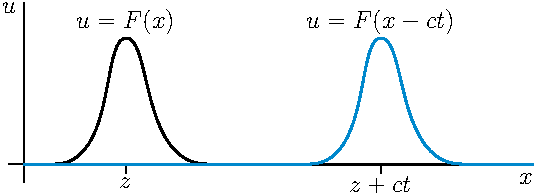
\includegraphics{fig/packet.pdf}
\end{center}
Similarly, $G(x+ct)$ represents a wave moving to the left with speed $c$.

\end{solution}

%%%%%%%%%%%%%%%%%%%%%%%%%%%%%%%%
\begin{question}
 Evaluate 
\begin{enumerate}[(a)]
\item
$\pdiff{y}{z}$\ if\ $e^{yz}-x^2 z \ln y = \pi$
\item
$\diff{y}{x}$\ if\ $F(x,y,x^2-y^2)=0$
\item
$\left(\pdiff{y}{x}\right)_u$\ if\
$xyuv=1$ and $x+y+u+v=0$ 
\end{enumerate}
\end{question}

\begin{hint}
For each part, first determine which variables $y$ is a function
of.
\end{hint}

\begin{answer}
(a) $\displaystyle\pdiff{y}{z}(x,z)
           =\frac{x^2 \ln y(x,z)-y(x,z)e^{y(x,z)\,z}}
                     {ze^{y(x,z)\,z}-\frac{x^2 z}{y(x,z)}}$

(b) $\displaystyle\diff{y}{x}(x)
=-\frac{F_1\big(x,y(x),x^2-y(x)^2\big)+2x\,F_3\big(x,y(x),x^2-y(x)^2\big)}
{F_2\big(x,y(x),x^2-y(x)^2\big)-2y(x)\,F_3\big(x,y(x),x^2-y(x)^2\big)}$

(c) $\displaystyle\left(\pdiff{y}{x}\right)_u\!\!(x,u)
=\frac{y(x,u)\,v(x,u)-x\,y(x,u)}{x\,y(x,u)-x\,v(x,u)}$

\end{answer}

\begin{solution}
(a)
We are told to evaluate $\pdiff{y}{z}$. So $y$ has to be a function of $z$
and possibly some other variables.
We are also told that $x$, $y$, and $z$ are related by the single equation
$e^{yz}-x^2 z \ln y = \pi$.
So we are to think of $x$ and $z$ as being independent variables and think of 
$y(x,z)$ as being determined by solving $e^{yz}-x^2 z \ln y = \pi$ for $y$ as a function of $x$ and $z$. That is, the function $y(x,z)$ obeys
\begin{equation*}
e^{y(x,z)\,z}-x^2 z \ln y(x,z) = \pi
\end{equation*}
for all $x$ and $z$.
Applying 
$\pdiff{}{z}$ to both sides of this equation gives
\begin{align*}
&\left[y(x,z)+z\pdiff{y}{z}(x,z)\right]e^{y(x,z)\,z}-x^2 \ln y(x,z)
-x^2 z\frac{1}{y(x,z)}\pdiff{y}{z}(x,z) = 0\\
\implies & \pdiff{y}{z}(x,z)
=\frac{x^2 \ln y(x,z)-y(x,z)e^{y(x,z)\,z}}{ze^{y(x,z)\,z}-\frac{x^2 z}{y(x,z)}}
\end{align*}

(b) 
We are told to evaluate $\diff{y}{x}$. So $y$ has to be a function of the single variable $x$. We are also told that $x$ and $y$ are related by $F(x,y,x^2-y^2)=0$. So the function $y(x)$ has to obey 
\begin{equation*}
F\big(x,y(x),x^2-y(x)^2\big)=0
\end{equation*}
for all $x$. Applying 
$\diff{}{x}$ to both sides of that equation and using the chain rule gives
\begin{align*}
&F_1\big(x,y(x),x^2-y(x)^2\big)\,\ \diff{x}{x} 
+F_2\big(x,y(x),x^2-y(x)^2\big)\ \diff{y}{x}(x)
\\&\hskip2in
+F_3\big(x,y(x),x^2-y(x)^2\big)\,\diff{}{x}\left[x^2-y(x)^2\right]= 0
\\
\implies &F_1\big(x,y(x),x^2-y(x)^2\big) +F_2\big(x,y(x),x^2-y(x)^2\big)\ \diff{y}{x}(x)
\\&\hskip2in
+F_3\big(x,y(x),x^2-y(x)^2\big)\,\left[2x-2y(x)\diff{y}{x}(x)\right]= 0
\\
\implies & \diff{y}{x}(x)
=-\frac{F_1\big(x,y(x),x^2-y(x)^2\big)+2x\,F_3\big(x,y(x),x^2-y(x)^2\big)}
{F_2\big(x,y(x),x^2-y(x)^2\big)-2y(x)\,F_3\big(x,y(x),x^2-y(x)^2\big)}
\end{align*}

(c) 
We are told to evaluate $\left(\pdiff{y}{x}\right)_u$, which is the partial
derivative of $y$ with respect to $x$ with $u$ being held fixed.
So $x$ and $u$ have to be independent variables and $y$ has to be a function of
$x$ and $u$.

Now the four variables $x$, $y$, $u$ and $v$ are related by the two equations
$xyuv=1$ and $x+y+u+v=0$. As $x$ and $u$ are to be independent variables,
$y=y(x,u)$, $v=v(x,u)$ are to be determined by solving $xyuv=1$, $x+y+u+v=0$
for $y$ and $v$ as functions of $x$ and $u$. That is 
\begin{align*}
x\,y(x,u)\,u\,v(x,u)&=1 \\
x+y(x,u)+u+v(x,u)&=0
\end{align*}
for all $x$ and $u$.
Applying 
$\pdiff{}{x}$ to both sides of both of these equations
gives
\begin{align*}
y\,u\,v\ +\ x\,\pdiff{y}{x}\,u\,v\ +\ x\,y\,u\,\pdiff{v}{x}&=0
\\
1+\pdiff{y}{x}+0+\pdiff{v}{x}&=0
\end{align*}
Substituting, $\pdiff{v}{x}=-1-\pdiff{y}{x}$,
from the second equation, into the first equation gives
\begin{align*}
y\,u\,v\ +\ x\,\pdiff{y}{x}\,u\,v-x\,y\,u
           \left(1+\pdiff{y}{x}\right)=0
\end{align*}
Now $u$ cannot be $0$ because $x\,y(x,u)\,u\,v(x,u)=1$. So
\begin{align*}
y\,v\ +\ x\,\pdiff{y}{x}\,v-x\,y\left(1+\pdiff{y}{x}\right)=0
\implies & \left(\pdiff{y}{x}\right)_u\!\!(x,u)
=\frac{y(x,u)\,v(x,u)-x\,y(x,u)}{x\,y(x,u)-x\,v(x,u)}
\end{align*}

\end{solution}
